% =====================================================================
%  KHÓA LUẬN TỐT NGHIỆP — Trường Đại học Công nghệ, ĐHQGHN
%  Học thói quen sinh hoạt của từng cư dân trong nhà thông minh nhiều người
%  Biên dịch trên Overleaf: Compiler = pdfLaTeX, Main document = main.tex
% =====================================================================
\documentclass[12pt,a4paper,oneside]{report}

% ---------- Tiếng Việt ----------
\usepackage[utf8]{inputenc}
\usepackage[T5]{fontenc}
\usepackage[english,vietnamese]{babel}  % ngôn ngữ chính: tiếng Việt (đứng cuối)
\usepackage{lmodern}

% ---------- Trang, khoảng cách ----------
\usepackage[left=3cm,right=2cm,top=2.5cm,bottom=2.5cm]{geometry}
\usepackage{setspace}
\onehalfspacing
\setlength{\parindent}{1cm}
\setlength{\parskip}{4pt}
\usepackage{indentfirst}
\raggedbottom

% ---------- Toán, bảng, hình ----------
\usepackage{amsmath,amssymb,amsthm}
\usepackage{graphicx}
\graphicspath{{figures/}}
\usepackage{booktabs}
\usepackage{array}
\usepackage{tabularx}
\usepackage{makecell}
\renewcommand{\cellalign}{cc}
\renewcommand{\theadalign}{cc}
\usepackage{multirow}
\usepackage{float}
\usepackage[font=small,labelfont=bf,labelsep=period]{caption}
\usepackage{subcaption}
\usepackage{xcolor}
\usepackage{tikz}
\usetikzlibrary{arrows.meta,positioning,calc}
\usepackage[ruled,vlined,linesnumbered]{algorithm2e}
\SetAlgorithmName{Thuật toán}{thuật toán}{Danh sách thuật toán}
\SetKwInput{KwIn}{Đầu vào}
\SetKwInput{KwOut}{Đầu ra}
\usepackage{enumitem}
\setlist{itemsep=2pt,topsep=4pt}

% ---------- Chương, mục (theo mẫu khóa luận UET) ----------
\usepackage{titlesec}
% Chương có số: dòng "Chương 1", dòng dưới là tên chương viết hoa.
\titleformat{\chapter}[display]
  {\normalfont\bfseries}{\huge\chaptertitlename\ \thechapter}{14pt}{\Huge\MakeUppercase}
\titlespacing*{\chapter}{0pt}{0pt}{28pt}
% Chương không số (Lời cảm ơn, Mục lục, Tài liệu tham khảo...): viết hoa, căn giữa.
\titleformat{name=\chapter,numberless}[block]
  {\normalfont\bfseries\Huge\filcenter}{}{0pt}{\MakeUppercase}
\titlespacing*{name=\chapter,numberless}{0pt}{0pt}{24pt}
\titleformat{\section}{\normalfont\Large\bfseries}{\thesection.}{0.5em}{}
\titleformat{\subsection}{\normalfont\large\bfseries}{\thesubsection.}{0.5em}{}

\usepackage{tocloft}
\renewcommand{\cftchapfont}{\bfseries}
\renewcommand{\cftchappagefont}{\bfseries}
\renewcommand{\cftchappresnum}{Chương\ }
\setlength{\cftchapnumwidth}{5.5em}

% ---------- Liên kết ----------
\usepackage[hidelinks,unicode]{hyperref}
\usepackage{url}

% ---------- Định nghĩa ----------
\theoremstyle{definition}
\newtheorem{definition}{Định nghĩa}[chapter]

% ---------- Thông tin chung ----------
\newcommand{\thesistitle}{HỌC THÓI QUEN SINH HOẠT CỦA TỪNG CƯ DÂN\\ TRONG NHÀ THÔNG MINH NHIỀU NGƯỜI\\ TỪ DỮ LIỆU CẢM BIẾN MÔI TRƯỜNG}
\newcommand{\thesistitleen}{LEARNING PER-RESIDENT DAILY HABITS\\ FROM AMBIENT SENSORS\\ IN MULTI-RESIDENT SMART HOMES}
\newcommand{\studentname}{Nguyễn Văn Biển}
\newcommand{\studentnameen}{Nguyen Van Bien}
\newcommand{\studentid}{23021477}
\newcommand{\studentclass}{QH-2023-I/CQ-I-CS3}
\newcommand{\supervisor}{TS. Vũ Thị Hồng Nhạn}
\newcommand{\supervisoren}{Dr. Vu Thi Hong Nhan}
\newcommand{\thesisyear}{2027}

% Ký hiệu dùng xuyên suốt
\newcommand{\Hb}{\mathcal{H}}
\newcommand{\Dd}{\mathcal{D}}

\begin{document}

% ---------------- Bìa ----------------
\pagenumbering{gobble}
% ---------------- Bìa (tiếng Việt), theo mẫu khóa luận UET ----------------
\begin{titlepage}
\centering
{\large\bfseries ĐẠI HỌC QUỐC GIA HÀ NỘI\\
TRƯỜNG ĐẠI HỌC CÔNG NGHỆ\par}
\vspace{4pt}
\rule{0.42\textwidth}{0.4pt}\par
\vspace{1.6cm}

\includegraphics[width=3.4cm]{uet_logo}\par
\vspace{1.6cm}
{\Large\bfseries \thesistitle\par}
\vspace{1cm}
{\large\bfseries KHÓA LUẬN TỐT NGHIỆP ĐẠI HỌC HỆ CHÍNH QUY\par}
\vspace{0.5cm}
{\large\bfseries Ngành: Khoa học máy tính\par}
\vfill
{\bfseries
\begin{tabular}{@{}l@{\hspace{0.8em}}c@{\hspace{0.8em}}l@{}}
Sinh viên & : & \studentname\\
Mã sinh viên & : & \studentid\\
Lớp & : & \studentclass\\
Cán bộ hướng dẫn & : & \supervisor
\end{tabular}\par}
\vspace{2cm}
{\bfseries HÀ NỘI -- \thesisyear\par}
\end{titlepage}

% ---------------- Bìa (tiếng Anh) ----------------
\begin{titlepage}
\centering
{\large\bfseries VIETNAM NATIONAL UNIVERSITY, HANOI\\
UNIVERSITY OF ENGINEERING AND TECHNOLOGY\par}
\vspace{4pt}
\rule{0.42\textwidth}{0.4pt}\par
\vspace{1.6cm}

\includegraphics[width=3.4cm]{uet_logo}\par
\vspace{1.6cm}
{\Large\bfseries \thesistitleen\par}
\vspace{1cm}
{\large\bfseries BACHELOR'S THESIS\par}
\vspace{0.5cm}
{\large\bfseries Major: Computer Science\par}
\vfill
{\bfseries
\begin{tabular}{@{}l@{\hspace{0.8em}}c@{\hspace{0.8em}}l@{}}
Student & : & \studentnameen\\
Student ID & : & \studentid\\
Class & : & \studentclass\\
Supervisor & : & \supervisoren
\end{tabular}\par}
\vspace{2cm}
{\bfseries HANOI -- \thesisyear\par}
\end{titlepage}


% ---------------- Phần đầu ----------------
\pagenumbering{roman}
\setcounter{page}{1}
\chapter*{Tóm tắt}
\addcontentsline{toc}{chapter}{Tóm tắt}

\textbf{Tóm tắt:} Nhà thông minh dùng cảm biến môi trường có thể học thói quen sinh hoạt của người ở mà
không cần camera hay thiết bị đeo --- nền tảng cho các ứng dụng chăm sóc người cao tuổi như nhắc uống
thuốc. Tuy nhiên, khi trong nhà có hai người, cảm biến không biết ai đã kích hoạt nó, nên các phương
pháp tìm thói quen dành cho nhà một người trộn lẫn thói quen của hai người. Khóa luận nghiên cứu bài toán
\emph{học thói quen của từng cư dân} từ luồng sự kiện cảm biến trộn lẫn. Khóa luận phát biểu hình thức
khái niệm thói quen theo từng người, hiện thực nó bằng thuật toán quét cửa sổ đếm theo ngày, xây dựng bộ
đánh giá ở mức thói quen, và so sánh năm cách tiếp cận --- hai baseline không nhãn (trong đó có phương
pháp của đề tài thực tập), một baseline tra bảng, Random Forest và Bi-GRU --- trên năm nhà của bộ dữ liệu
CASAS, đánh giá theo thứ tự thời gian. Trên ba nhà hai người, nhận dạng (người, hoạt động) rồi áp định
nghĩa thói quen đạt F1 thói quen 0,50--0,71 (Random Forest), so với 0,22--0,33 của phương pháp theo vùng;
ở nhà Cairo, mô hình tìm đủ 6/6 thói quen gắn với từng người, kể cả thói quen uống thuốc vốn trùng giờ và
trùng cảm biến với bữa sáng. Phân tích lỗi lan truyền bằng cách làm nhiễu nhãn có kiểm soát cho thấy thói
quen chịu được lệch giờ nhỏ và nhận thừa ngẫu nhiên, nhưng nhạy với bỏ sót, nhầm người và lỗi có hệ
thống. Thí nghiệm phát hiện ngày bỏ thuốc trên dữ liệu có cài bất thường cho thấy Bi-GRU phát hiện được
9/10 ngày nhưng còn nhiều báo động nhầm, trong khi cách tiếp cận theo vùng không phát hiện được ngày nào.

\textbf{Từ khóa:} nhà thông minh, nhiều cư dân, cảm biến môi trường, khai phá thói quen, nhận dạng hoạt
động, phát hiện bất thường.

\vspace{1cm}
\begin{otherlanguage}{english}
\noindent\textbf{Abstract:} Smart homes with ambient sensors can learn the daily habits of their
residents without cameras or wearables --- a foundation for elderly-care applications such as medication
reminders. When two people share a home, however, the sensors do not know who triggered them, and habit
discovery methods designed for single-resident homes mix the habits of both. This thesis studies how to
\emph{learn per-resident habits} from such a mixed sensor stream. It formally defines a per-resident habit,
implements the definition as a day-counting window-scan algorithm, builds a habit-level evaluation
protocol, and compares five approaches --- two label-free baselines (including the author's internship
method), a lookup baseline, Random Forest and Bi-GRU --- on five CASAS homes under a chronological split.
On the three two-resident homes, recognising (resident, activity) and then applying the habit definition
reaches a habit F1 of 0.50--0.71 (Random Forest) versus 0.22--0.33 for the zone-based approach; in the
Cairo home it recovers all 6/6 per-resident habits, including a medication habit that shares its time and
sensors with breakfast. A controlled label-corruption analysis shows that habits tolerate small time
shifts and random false positives but are sensitive to missed occurrences, resident swaps and systematic
errors. In a missed-medication detection experiment with injected anomalies, Bi-GRU detects 9 of 10
skipped days at the cost of frequent false alarms, while the zone-based approach detects none.

\noindent\textbf{Keywords:} smart home, multi-resident, ambient sensors, habit mining, activity
recognition, anomaly detection.
\end{otherlanguage}

\chapter*{Lời cảm ơn}
\addcontentsline{toc}{chapter}{Lời cảm ơn}

Trước hết, em xin bày tỏ lòng biết ơn sâu sắc tới TS. Vũ Thị Hồng Nhạn, người đã tận tình
định hướng, góp ý và đồng hành cùng em từ đợt thực tập đến khi thực hiện khóa luận này. Những
nhận xét của cô giúp em học được cách tiếp cận một bài toán nghiên cứu một cách bài bản: từ đọc
tài liệu, xác định phạm vi, thiết kế thực nghiệm đến đánh giá kết quả một cách trung thực.

Em xin cảm ơn các thầy cô Trường Đại học Công nghệ, Đại học Quốc gia Hà Nội đã trang bị cho em
nền tảng kiến thức trong suốt những năm học tập.

Em cũng xin cảm ơn nhóm CASAS, Đại học Bang Washington, đã công bố công khai các bộ dữ liệu nhà
thông minh được sử dụng trong khóa luận.

Cuối cùng, em xin cảm ơn gia đình và bạn bè đã luôn động viên, ủng hộ em.

Do thời gian và kiến thức còn hạn chế, khóa luận khó tránh khỏi thiếu sót. Em rất mong nhận được
góp ý của thầy cô để hoàn thiện hơn.

\vspace{1cm}
\begin{flushright}
\begin{tabular}{c}
Hà Nội, ngày \quad tháng \quad năm \thesisyear\\
\textbf{Sinh viên}\\[2.2cm]
\studentname
\end{tabular}
\end{flushright}

\chapter*{Lời cam đoan}
\addcontentsline{toc}{chapter}{Lời cam đoan}

Tôi là \studentname, mã sinh viên \studentid, lớp \studentclass, xin cam đoan khóa luận
``\textit{Học thói quen sinh hoạt của từng cư dân trong nhà thông minh nhiều người từ dữ liệu
cảm biến môi trường}'' là công trình nghiên cứu của riêng tôi, được thực hiện dưới sự hướng dẫn
của \supervisor.

Các số liệu và kết quả trình bày trong khóa luận là trung thực, được sinh ra từ mã nguồn đi kèm
và có thể tái lập. Mọi thông tin tham khảo từ công trình khác đều được trích dẫn đầy đủ. Nếu có
bất kỳ sai phạm nào, tôi xin hoàn toàn chịu trách nhiệm trước Hội đồng và Nhà trường.

\textbf{Về việc sử dụng công cụ trí tuệ nhân tạo.} Trong quá trình thực hiện, tôi có sử dụng
trợ lý AI (Claude) để hỗ trợ tra cứu tài liệu, rà soát mã nguồn và trình bày văn bản. Ý tưởng
nghiên cứu, các quyết định về phạm vi và phương pháp, việc kiểm tra kết quả thực nghiệm và nội
dung cuối cùng của khóa luận do tôi xem xét, kiểm chứng và chịu trách nhiệm.

\vspace{1cm}
\begin{flushright}
\begin{tabular}{c}
Hà Nội, ngày \quad tháng \quad năm \thesisyear\\
\textbf{Sinh viên}\\[2.2cm]
\studentname
\end{tabular}
\end{flushright}


\tableofcontents
\listoffigures
\listoftables
\chapter*{Danh mục từ viết tắt và thuật ngữ}
\addcontentsline{toc}{chapter}{Danh mục từ viết tắt và thuật ngữ}

{\renewcommand{\arraystretch}{1.25}
\noindent\begin{tabularx}{\textwidth}{@{}>{\bfseries}p{2.2cm}>{\raggedright\arraybackslash}X>{\raggedright\arraybackslash}X@{}}
\toprule
Viết tắt & \textbf{Tiếng Anh} & \textbf{Tiếng Việt}\\
\midrule
ARI & Adjusted Rand Index & Chỉ số Rand hiệu chỉnh\\
Bi-GRU & Bidirectional Gated Recurrent Unit & Mạng hồi quy có cổng hai chiều\\
CASAS & Center for Advanced Studies in Adaptive Systems & Dự án nhà thông minh của Đại học Bang Washington\\
CPD & Change Point Detection & Phát hiện điểm thay đổi\\
DBSCAN & Density-Based Spatial Clustering of Applications with Noise & Phân cụm theo mật độ có nhiễu\\
F1 & F1-score & Trung bình điều hòa của độ chính xác và độ phủ\\
HAR & Human Activity Recognition & Nhận dạng hoạt động của con người\\
HDBSCAN & Hierarchical DBSCAN & DBSCAN phân cấp\\
LLM & Large Language Model & Mô hình ngôn ngữ lớn\\
P, R & Precision, Recall & Độ chính xác, độ phủ\\
PIR & Passive Infrared & Cảm biến hồng ngoại thụ động (chuyển động)\\
RF & Random Forest & Rừng ngẫu nhiên\\
RQ & Research Question & Câu hỏi nghiên cứu\\
\bottomrule
\end{tabularx}\par}

\vspace{0.8cm}
\noindent{\large\bfseries Một số thuật ngữ dùng trong khóa luận}
\begin{itemize}
  \item \textbf{Sự kiện cảm biến}: một dòng nhật ký ``thời điểm $t$, cảm biến $s$, giá trị $v$''.
  \item \textbf{Lần thực hiện} (episode): một đoạn thời gian $[t^{s}, t^{e}]$ trong đó một người thực hiện
        một hoạt động.
  \item \textbf{Thói quen}: tập các lần thực hiện cùng một hoạt động, bởi cùng một người, bắt đầu quanh
        cùng một giờ, lặp lại ở ít nhất một nửa số ngày (Định nghĩa~\ref{def:habit}).
  \item \textbf{Thói quen đáp án}: thói quen thu được khi áp định nghĩa lên nhãn thật; chỉ dùng để đánh giá.
  \item \textbf{Vùng}: nhóm cảm biến gần nhau, rút ra từ dữ liệu, đóng vai trò ``phòng''.
  \item \textbf{Vệt} (track): chuỗi sự kiện được cho là do cùng một người gây ra.
  \item \textbf{Nhãn thật (Oracle)}: khai phá thói quen trực tiếp trên nhãn thật; là giới hạn trên của
        mọi phương pháp.
\end{itemize}


% ---------------- Nội dung ----------------
\clearpage
\pagenumbering{arabic}
\setcounter{page}{1}
\chapter{Giới thiệu}
\label{chap:intro}

\section{Bối cảnh và động lực}

Việt Nam đang già hóa dân số với tốc độ nhanh. Theo số liệu năm 2024 của Tổng cục Thống kê, cả
nước có khoảng 14,2 triệu người cao tuổi, chiếm khoảng 14\% dân số, và dự kiến bước vào giai
đoạn dân số già vào khoảng năm 2034--2036~\cite{vnexpress2024tuoigia}. Việc chăm sóc người cao
tuổi hiện chủ yếu do người thân trong gia đình đảm nhận, trong khi dịch vụ chăm sóc cộng đồng
còn hạn chế. Bối cảnh đó tạo ra nhu cầu về những công cụ giúp người thân theo dõi sinh hoạt
hằng ngày của người cao tuổi từ xa, với chi phí thấp và không xâm phạm quyền riêng tư.

Nhà thông minh dùng \textbf{cảm biến môi trường} --- cảm biến chuyển động hồng ngoại (PIR), cảm
biến cửa, cảm biến nhiệt độ --- là một hướng đáp ứng nhu cầu đó: thiết bị rẻ, không cần camera,
không bắt người dùng đeo thiết bị~\cite{cook2013casas,bouchabou2021survey}. Từ nhật ký sự kiện
của các cảm biến, hệ thống có thể học được \textbf{thói quen} của người ở: thức dậy lúc mấy giờ,
ăn sáng khi nào, có uống thuốc đều đặn không. Thói quen là nền tảng cho nhiều ứng dụng: nhắc nhở
khi quên uống thuốc --- một vấn đề có thật khi tỉ lệ tuân thủ điều trị bệnh mạn tính trung bình
chỉ khoảng 50\%~\cite{who2003adherence} ---, cảnh báo khi sinh hoạt thay đổi bất thường, hay tự
động hóa thiết bị theo nhịp sống của từng người.

Trong đợt thực tập trước đó, tác giả đã xây dựng một phương pháp không giám sát để tìm thói quen
từ dữ liệu cảm biến: gom sự kiện thành \emph{phiên} (một lần ở liên tục trong một phòng), biểu
diễn giờ trong ngày trên vòng tròn và phân cụm bằng DBSCAN~\cite{ester1996dbscan}. Phương pháp
tìm lại đủ 12/12 thói quen cài sẵn trên dữ liệu mô phỏng và 5 thói quen trên dữ liệu thật của
một người sống một mình. Tuy nhiên, phương pháp đó --- cũng như phần lớn nghiên cứu về khai phá
mẫu sinh hoạt --- ngầm giả định \textbf{trong nhà chỉ có một người}.

Giả định này không đúng với thực tế. Người cao tuổi thường sống cùng vợ hoặc chồng, hoặc cùng con
cháu. Khi trong nhà có hai người, cảm biến môi trường \emph{không biết ai đã kích hoạt nó}: các
sự kiện của hai người trộn vào một luồng duy nhất~\cite{benmansour2015survey,wang2021smrt}. Luận
án tiến sĩ của Dong Chen~\cite{chen2021thesis} --- tài liệu định hướng chính của khóa luận ---
đã chỉ ra rằng nhận dạng hoạt động trong nhà nhiều người khó hơn hẳn nhà một người, và đề xuất
các kỹ thuật phân đoạn, phân lớp và học trực tuyến cho bài toán này. Nhưng luận án đó dừng ở việc
nhận dạng \emph{hoạt động đang diễn ra}; chính tác giả nêu trong phần hạn chế rằng các phương
pháp ``chỉ nhận ra hoạt động hiện tại'' và chưa hướng tới hành vi dài hạn.

\section{Bài toán và ví dụ minh họa}
\label{sec:intro-example}

Xét bộ dữ liệu CASAS Cairo~\cite{casas2025zenodo}: một cặp vợ chồng (ký hiệu R1, R2) sống trong
căn nhà ba tầng gắn 27 cảm biến chuyển động, được ghi nhận trong 57 ngày. Bảng~\ref{tab:cairo-morning}
thống kê bốn hoạt động buổi sáng.

\begin{table}[htbp]
\centering
\caption{Bốn hoạt động buổi sáng ở nhà Cairo (thống kê trên nhãn thật của toàn bộ dữ liệu)}
\label{tab:cairo-morning}
\begin{tabular}{llcl}
\toprule
Hoạt động & Người & Giờ trung vị & Cảm biến kích hoạt nhiều nhất \\
\midrule
Thức dậy & R1 & 06:44 & M005, M001 (tầng trên) \\
Thức dậy & R2 & 07:04 & M005, M009 (tầng trên) \\
\textbf{Uống thuốc} & \textbf{R2} & \textbf{07:20} & \textbf{M021, M024 (bếp)} \\
Ăn sáng & chung & 07:29 & M024, M021 (bếp) \\
\bottomrule
\end{tabular}
\end{table}

Thói quen uống thuốc của R2 và bữa sáng chung dùng đúng những cảm biến bếp giống nhau và chỉ cách
nhau khoảng 10 phút. Một phương pháp chỉ nhìn ``phòng nào, mấy giờ'' như ở đợt thực tập không thể
tách hai thói quen này; thực nghiệm ở Chương~\ref{chap:exp} cho thấy nó còn gộp mọi bữa ăn trong
ngày của vùng bếp vào \emph{một} cụm duy nhất. Muốn biết ``R2 có uống thuốc lúc khoảng 7 giờ mỗi
sáng không'', hệ thống phải (i) gán được các đoạn sự kiện cho đúng người và đúng hoạt động, rồi
(ii) từ đó rút ra thói quen của từng người.

Khóa luận giải bài toán: \textbf{từ luồng sự kiện cảm biến trộn lẫn của nhà hai người, tìm đúng
thói quen của từng người}, và chứng minh thói quen tìm được dùng được để \textbf{phát hiện ngày bỏ
thuốc}.

\section{Câu hỏi nghiên cứu}

Khóa luận trả lời ba câu hỏi nghiên cứu:

\begin{description}[leftmargin=1.3cm,style=sameline]
  \item[RQ1] Gán các đoạn sự kiện cảm biến cho \emph{đúng người và đúng hoạt động} chính xác đến
  đâu, khi chỉ dùng cảm biến môi trường và đánh giá theo thứ tự thời gian?
  \item[RQ2] Từ kết quả của RQ1, thói quen của từng người tìm được \emph{đúng đến đâu} so với thói
  quen đáp án? Lỗi ở khâu nhận dạng --- bỏ sót, lệch giờ, nhận nhầm, \emph{nhầm người} --- lan
  truyền sang thói quen như thế nào? (Câu hỏi trung tâm.)
  \item[RQ3] Thói quen học được có phát hiện được \emph{ngày bỏ thuốc} không, và tốt hơn cách tiếp
  cận theo phòng đến đâu?
\end{description}

\section{Mục tiêu và phạm vi}

\textbf{Mục tiêu.} Xây dựng và đánh giá một quy trình đầu--cuối đi từ nhật ký cảm biến thô tới
danh sách thói quen của từng người; đưa ra định nghĩa đo được của khái niệm ``thói quen theo từng
người'' cùng bộ chỉ số đánh giá ở mức thói quen.

\textbf{Phạm vi} (được chốt trước khi thực hiện để tránh thay đổi giữa chừng):
\begin{itemize}
  \item \emph{Trong phạm vi:} nhà hai người; dữ liệu công khai CASAS (Cairo, Tulum1, Tulum2 là nhà
  hai người; Milan, Aruba là nhà một người dùng để đối chứng); đánh giá ngoại tuyến, chia dữ liệu
  theo ngày; các phương pháp baseline và mô hình học trình bày ở Chương~\ref{chap:method}.
  \item \emph{Ngoài phạm vi:} camera, thiết bị đeo; mô hình ngôn ngữ lớn và mô hình nền; nhà từ ba
  người trở lên; tự thu thập dữ liệu; gán người cho \emph{từng} sự kiện cảm biến (dữ liệu không
  có nhãn này); học trực tuyến; dự đoán hành động tiếp theo; ứng dụng nhắc nhở thật, điều khiển
  thiết bị, robot.
\end{itemize}

\section{Đóng góp}

\begin{enumerate}
  \item \textbf{Định nghĩa và thuật toán thói quen.} Phát biểu hình thức khái niệm thói quen theo
  từng người và hiện thực nó thành thuật toán \emph{quét cửa sổ} đếm theo ngày, khắc phục hiện
  tượng ``chuỗi hóa'' của DBSCAN mà đề tài thực tập gặp phải.
  \item \textbf{Bộ đánh giá ở mức thói quen.} Thói quen đáp án, phép so khớp một--một bằng thuật
  toán Hungary và các chỉ số precision, recall, F1, sai số giờ, sai số tần suất; tách riêng đánh
  giá thói quen gắn với từng người.
  \item \textbf{So sánh có kiểm soát} năm cách tiếp cận (hai baseline không nhãn, một baseline tra
  bảng, Random Forest, Bi-GRU) và giới hạn trên Oracle trên năm nhà, đánh giá theo thứ tự thời gian.
  \item \textbf{Phân tích lỗi lan truyền}: làm nhiễu nhãn thật có kiểm soát để đo thói quen nhạy
  với từng loại lỗi nhận dạng đến đâu, kể cả lỗi \emph{tráo người} đặc trưng của nhà nhiều người.
  \item \textbf{Thí nghiệm ứng dụng} phát hiện ngày bỏ thuốc trên dữ liệu thật có cài bất thường.
  \item Mã nguồn mở, có kiểm thử, tái lập toàn bộ số liệu bằng một lệnh.
\end{enumerate}

\section{Ý nghĩa khoa học và thực tiễn}

\textbf{Về khoa học}, khóa luận nối hai hướng nghiên cứu đang tách rời: nhận dạng hoạt động trong
nhà nhiều người~\cite{chen2021thesis,wang2021smrt,chen2026mdp} và khai phá mẫu sinh hoạt vốn mới
được kiểm chứng trên nhà một người~\cite{karpekov2025discover}. Việc đo lỗi lan truyền cho biết
khâu nhận dạng cần tốt đến đâu thì thói quen mới đáng tin --- thông tin hữu ích để quyết định đầu
tư cho khâu nào.

\textbf{Về thực tiễn}, thói quen theo từng người là lớp nền cho các ứng dụng chăm sóc người cao
tuổi trong những ngôi nhà có nhiều hơn một người --- trường hợp phổ biến nhưng ít được nghiên cứu.
Chỉ dùng cảm biến môi trường giúp giải pháp rẻ và tôn trọng quyền riêng tư.

\textbf{Giới hạn cần nói rõ}: dữ liệu thu ở Mỹ giai đoạn 2009--2011 với tối đa hai người; bất
thường trong RQ3 là bất thường \emph{cài vào}; khóa luận không khẳng định hệ thống dùng được ngay
cho nhà thật ở Việt Nam.

\section{Cấu trúc khóa luận}

\begin{itemize}
  \item \textbf{Chương~\ref{chap:background}} tổng quan nhà thông minh, nhận dạng hoạt động, bài
  toán nhà nhiều người, khai phá mẫu sinh hoạt và các kiến thức nền; định vị khoảng trống.
  \item \textbf{Chương~\ref{chap:method}} phát biểu hình thức bài toán, định nghĩa thói quen và
  trình bày toàn bộ quy trình cùng cách đánh giá.
  \item \textbf{Chương~\ref{chap:exp}} trình bày dữ liệu, thiết lập và kết quả thực nghiệm cho ba
  câu hỏi nghiên cứu, ablation và phân tích độ nhạy.
  \item \textbf{Chương~\ref{chap:conclusion}} tổng kết, nêu hạn chế và hướng phát triển.
\end{itemize}

\chapter{Tổng quan và kiến thức nền}
\label{chap:background}

Chương này trình bày bối cảnh kỹ thuật của khóa luận: nhà thông minh dùng cảm biến môi trường
(mục~\ref{sec:bg-smarthome}), quy trình nhận dạng hoạt động (mục~\ref{sec:bg-har}), bài toán nhà
nhiều người với trọng tâm là luận án của Chen~\cite{chen2021thesis} (mục~\ref{sec:bg-multi}),
các hướng khai phá mẫu sinh hoạt và theo dõi thay đổi hành vi (mục~\ref{sec:bg-routine}), xu hướng
dùng mô hình ngôn ngữ (mục~\ref{sec:bg-llm}), các kiến thức nền được dùng trong khóa luận
(mục~\ref{sec:bg-tools}) và cuối cùng là khoảng trống mà khóa luận hướng tới
(mục~\ref{sec:bg-gap}).

\section{Nhà thông minh và cảm biến môi trường}
\label{sec:bg-smarthome}

Theo cách phân loại phổ biến, cảm biến dùng cho nhận dạng hoạt động gồm năm nhóm: camera, thiết bị
đeo, điện thoại, âm thanh và cảm biến môi trường~\cite{chen2021thesis,bouchabou2021survey}. Camera
cho thông tin giàu nhất nhưng đắt và xâm phạm riêng tư; thiết bị đeo rẻ hơn nhưng người cao tuổi
thường ngại đeo hoặc quên đeo. \emph{Cảm biến môi trường} --- gắn cố định trong nhà --- được xem là
hướng hợp lý cho chăm sóc tại nhà vì không xâm nhập, rẻ và dễ lắp đặt~\cite{chen2021thesis}.

Dự án CASAS của Đại học Bang Washington~\cite{cook2013casas} là nguồn dữ liệu chuẩn của lĩnh vực.
Mỗi nhà gắn vài chục cảm biến: cảm biến chuyển động (ký hiệu \texttt{M}, giá trị \texttt{ON/OFF}),
cảm biến cửa (\texttt{D}, \texttt{OPEN/CLOSE}) và cảm biến nhiệt độ (\texttt{T}). Mỗi dòng dữ liệu
là một \emph{sự kiện}: \texttt{2009-06-10 07:12:05 M021 ON}. Một số dòng kèm nhãn do người chú
thích ghi, dạng \texttt{R2\_Take\_Medicine begin/end}, đánh dấu đầu và cuối một lần thực hiện hoạt
động. Đặc điểm quan trọng: dữ liệu \emph{thưa} (cảm biến chỉ kích hoạt khi có chuyển động),
\emph{không đều} theo thời gian và \emph{vô danh} --- không ghi ai đã kích hoạt cảm biến.

\section{Nhận dạng hoạt động từ cảm biến môi trường}
\label{sec:bg-har}

Chen~\cite{chen2021thesis} tổng kết quy trình nhận dạng hoạt động dựa trên dữ liệu thành bốn bước:
\emph{thu thập dữ liệu} $\rightarrow$ \emph{tiền xử lý và phân đoạn} $\rightarrow$ \emph{phân lớp}
$\rightarrow$ \emph{suy luận và đánh giá}.

\textbf{Phân đoạn.} Chuỗi sự kiện liên tục phải được cắt thành các đoạn để phân lớp. Ba cách cơ
bản là cửa sổ trượt cố định theo thời gian, cửa sổ cố định theo số sự kiện và cửa sổ động dựa trên
tương quan giữa cảm biến~\cite{chen2021thesis,krishnan2014streaming}. Krishnan và
Cook~\cite{krishnan2014streaming} đề xuất gán nhãn cho \emph{từng sự kiện} dựa trên cửa sổ các sự
kiện ngay trước nó --- cách làm phù hợp với dữ liệu dạng luồng và được khóa luận kế thừa.
Phát hiện điểm thay đổi (CPD)~\cite{aminikhanghahi2017cpd} là một cách khác để tìm ranh giới hoạt
động.

\textbf{Phân lớp.} Các mô hình truyền thống gồm Naive Bayes, mô hình Markov ẩn, trường ngẫu nhiên
có điều kiện, cây quyết định, SVM và rừng ngẫu nhiên~\cite{breiman2001rf}; các mô hình học sâu gồm
CNN và nhất là các mạng hồi quy LSTM, GRU và biến thể hai chiều~\cite{cho2014gru,schuster1997brnn}.
Thực nghiệm của Chen cho thấy mạng hồi quy thường vượt các mô hình khác trên dữ liệu chuỗi thời
gian~\cite{chen2021thesis}.

\textbf{Đánh giá.} Các chỉ số thường dùng là accuracy, precision, recall và F1. Một điểm cần lưu ý
về phương pháp luận: nhiều công trình, kể cả~\cite{chen2021thesis}, dùng kiểm định chéo 10 lần mà
không nói rõ có chia theo thời gian hay không. Với dữ liệu chuỗi thời gian, nếu chia ngẫu nhiên thì
các cửa sổ liền kề --- gần như giống nhau --- rơi vào cả tập huấn luyện lẫn tập kiểm tra, làm kết
quả cao hơn thực tế. Khóa luận chia dữ liệu \emph{theo ngày, theo thứ tự thời gian} để tránh rủi ro
này.

\section{Nhà nhiều người}
\label{sec:bg-multi}

\subsection{Thách thức}

Khi có từ hai người trở lên, các sự kiện của họ trộn vào một luồng theo thứ tự thời
gian~\cite{benmansour2015survey}. Bên cạnh hoạt động tuần tự, xen kẽ và đồng thời của một người,
xuất hiện thêm hoạt động \emph{song song} (mỗi người làm một việc ở một nơi) và \emph{cộng tác}
(cùng làm một việc)~\cite{chen2021thesis}. Hệ thống không chỉ phải biết ``đang có hoạt động gì'' mà
còn phải biết ``ai đang làm''~\cite{singla2010multiresident}.

\subsection{Luận án của Chen (2021)}

Luận án tiến sĩ của Dong Chen~\cite{chen2021thesis} là tài liệu định hướng chính của khóa luận. Luận
án giải ba bài toán con:
\begin{enumerate}
  \item \textbf{Phân đoạn} (Chương 3 của luận án, công bố trên IEEE Internet of Things
  Journal~\cite{chen2021fcmcpd}): gom cảm biến theo \emph{vị trí} bằng Fuzzy C-means --- hai sự kiện
  liên tiếp ở hai vùng khác nhau khó do cùng một người gây ra --- rồi dùng CPD để tìm điểm chuyển
  hoạt động trong từng nhóm.
  \item \textbf{Phân lớp} (Chương 4): mô hình TRANS-BiGRU kết hợp Transformer với Bi-GRU, so sánh với
  khoảng 15 mô hình học máy và học sâu trên CASAS và ARAS~\cite{alemdar2013aras}.
  \item \textbf{Học trực tuyến} (Chương 5): rừng ngẫu nhiên thích nghi kèm bộ phát hiện trôi khái
  niệm (LED-ARF) cho dữ liệu đến liên tục.
\end{enumerate}
Chính luận án nêu ba hạn chế: dữ liệu chỉ có hai người và hoạt động đơn giản; hiệu năng còn khoảng
cách để cải thiện; và các phương pháp \emph{chỉ nhận ra hoạt động hiện tại}, chưa dự đoán hay phát
hiện bất thường. Khóa luận kế thừa \emph{khung} của luận án (tách người $\rightarrow$ nhận dạng) và
\emph{ý tưởng} dùng vị trí để tách người, nhưng không tái hiện các mô hình của luận án; thay vào đó,
khóa luận đi tiếp theo hướng luận án còn bỏ ngỏ: từ nhận dạng sang \emph{hành vi dài hạn}.

\subsection{Gán sự kiện cho từng người}

Bài toán ``sự kiện này do ai gây ra'' được gọi là \emph{liên kết dữ liệu} (data association) hay
\emph{theo dõi nhiều cư dân}. Crandall và Cook~\cite{crandall2009coping} dùng luật dựa trên đồ thị
kề của cảm biến; Wang và Cook~\cite{wang2021smrt} (sMRT) vector hóa cảm biến để theo dõi nhiều người
mà không cần sơ đồ nhà. Gần đây, Chen, Cumin và cộng sự~\cite{chen2026mdp} mô hình hóa bài toán như
một quá trình quyết định Markov, huấn luyện bằng học bắt chước với Transformer nhỏ hoặc mô hình ngôn
ngữ lớn; công trình này cho thấy gán sai người làm sai các chỉ số sức khỏe phía sau, như thời lượng
hoạt động. Các công trình trên đánh giá ở mức \emph{sự kiện} hoặc \emph{vệt}; chưa công trình nào
đánh giá tác động lên \emph{thói quen}.

\section{Khai phá mẫu sinh hoạt và thay đổi hành vi}
\label{sec:bg-routine}

Một hướng khác không hỏi ``hoạt động hiện tại là gì'' mà hỏi ``sinh hoạt thường ngày như thế nào''.
Duckworth và cộng sự~\cite{duckworth2019unsupervised} cho robot di động tự học các lớp hoạt động
không cần nhãn; bộ dữ liệu dài hạn của dự án STRANDS~\cite{coppola2016temporal} là dữ liệu thật của
đề tài thực tập. DISCOVER~\cite{karpekov2025discover} học biểu diễn tự giám sát rồi phân cụm để tìm
``mẫu sinh hoạt hằng ngày'', chỉ cần gán nhãn rất ít cụm --- nhưng chỉ kiểm chứng trên nhà một người.
X-BCD~\cite{civitarese2026xbcd} phát hiện thay đổi hành vi theo thời gian và giải thích cho bác sĩ.

Đề tài thực tập của tác giả thuộc hướng này: thói quen được định nghĩa là nhóm phiên cùng phòng, bắt
đầu lệch nhau không quá khoảng 30 phút, lặp lại ở ít nhất 50\% số ngày, và được tìm bằng DBSCAN
trên không gian giờ vòng tròn. Hạn chế được ghi nhận khi đó: một hoạt động kéo dài cả buổi (ngồi
phòng khách) bị DBSCAN nối thành một khung giờ rất rộng, và dữ liệu thật chỉ có một người.

\section{Xu hướng mô hình ngôn ngữ và mô hình nền}
\label{sec:bg-llm}

Từ 2024, nhiều công trình chuyển chuỗi cảm biến thành văn bản để dùng mô hình ngôn ngữ: ADL-LLM nhận
dạng hoạt động không cần nhãn huấn luyện~\cite{civitarese2024adlllm}; TDOST mô tả mỗi lần cảm biến
kích hoạt bằng câu chữ để chuyển mô hình sang nhà khác~\cite{thukral2024tdost}; một số công trình
dùng biểu diễn ngôn ngữ thay vì sinh văn bản~\cite{dhekane2025prompt}; DomusFM là mô hình nền đầu
tiên huấn luyện riêng cho dữ liệu nhà thông minh~\cite{fiori2026domusfm}. Bộ dữ liệu MuRAL~\cite{chen2025mural}
(2--4 người, chú thích bằng ngôn ngữ tự nhiên) cho thấy các mô hình ngôn ngữ hiện tại vẫn gặp khó
khi phải phân biệt ai kích hoạt cảm biến. Dự đoán hoạt động tiếp theo bằng mô hình ngôn ngữ cũng đã
được thử nghiệm~\cite{doctorarastoo2026prediction}. Các hướng này nằm \emph{ngoài phạm vi} khóa luận
và được nhắc lại trong phần hướng phát triển.

\section{Kiến thức nền}
\label{sec:bg-tools}

\subsection{Thống kê vòng tròn}
Giờ trong ngày là đại lượng tuần hoàn: 23:50 và 00:10 chỉ cách nhau 20 phút nhưng nếu biểu diễn bằng
số thực (23,83 và 0,17) thì cách nhau gần một ngày. Cách xử lý chuẩn~\cite{fisher1993circular} là
đặt giờ $h$ lên vòng tròn với góc $\theta = 2\pi h/24$. Trung bình vòng tròn của các giờ
$h_1,\dots,h_n$ là
\begin{equation}
  \bar h = \frac{24}{2\pi}\,\operatorname{atan2}\Big(\tfrac1n\textstyle\sum_i \sin\theta_i,\;
  \tfrac1n\sum_i \cos\theta_i\Big) \bmod 24,
\end{equation}
và chênh lệch có dấu giữa hai giờ là $\delta(a,b) = \big((a-b+12) \bmod 24\big) - 12 \in [-12, 12)$.

\subsection{Phân cụm theo mật độ}
DBSCAN~\cite{ester1996dbscan} gom các điểm có ít nhất \texttt{min\_samples} láng giềng trong bán
kính $\varepsilon$ thành cụm, các điểm còn lại là nhiễu; không cần biết trước số cụm. Nhược điểm
liên quan trực tiếp tới khóa luận: các điểm có thể ``nối chuỗi'' qua nhau, nên một hoạt động diễn
ra rải rác cả ngày tạo thành một cụm kéo dài cả ngày. HDBSCAN~\cite{campello2013hdbscan} xây cây
phân cấp mật độ và chọn cụm ổn định nhất, không cần $\varepsilon$ nhưng vì thế cũng không có khái
niệm ``lệch không quá 30 phút''.

\subsection{Rừng ngẫu nhiên và mạng hồi quy}
Rừng ngẫu nhiên~\cite{breiman2001rf} kết hợp nhiều cây quyết định học trên các mẫu bootstrap và tập
con đặc trưng ngẫu nhiên; ổn định, ít cần tinh chỉnh và hỗ trợ trực tiếp bài toán nhiều đầu ra. GRU
\cite{cho2014gru} là mạng hồi quy có cổng cập nhật và cổng đặt lại; phiên bản hai chiều
\cite{schuster1997brnn} đọc chuỗi theo cả hai chiều rồi ghép trạng thái ẩn.

\subsection{Phân cụm phổ}
Phân cụm phổ~\cite{vonluxburg2007spectral} dùng các vector riêng của ma trận Laplacian chuẩn hóa
$L = I - D^{-1/2} A D^{-1/2}$ của đồ thị tương đồng $A$. Số cụm có thể chọn theo \emph{khoảng cách
trị riêng}: $k$ là vị trí có bước nhảy lớn nhất giữa hai trị riêng liên tiếp nhỏ nhất.

\subsection{Bài toán ghép cặp}
Để so khớp một--một hai tập phần tử theo một ma trận chi phí, thuật toán Hungary~\cite{kuhn1955hungarian}
tìm cách ghép có tổng chi phí nhỏ nhất trong thời gian đa thức.

\section{Khoảng trống nghiên cứu và vị trí của khóa luận}
\label{sec:bg-gap}

Bảng~\ref{tab:gap} đặt khóa luận cạnh các công trình gần nhất.

\begin{table}[htbp]
\centering
\caption{Vị trí của khóa luận so với các công trình liên quan}
\label{tab:gap}
\small
\begin{tabularx}{\textwidth}{>{\raggedright\arraybackslash}X ccc}
\toprule
Công trình & Nhà nhiều người & Đầu ra là thói quen & Đánh giá mức thói quen \\
\midrule
Chen 2021~\cite{chen2021thesis,chen2021fcmcpd} & \checkmark & -- & -- \\
sMRT 2021~\cite{wang2021smrt}; MDP 2026~\cite{chen2026mdp} & \checkmark & -- & -- \\
DISCOVER 2025~\cite{karpekov2025discover} & -- & \checkmark & một phần \\
X-BCD 2026~\cite{civitarese2026xbcd} & -- & thay đổi hành vi & -- \\
Đề tài thực tập & -- & \checkmark & \checkmark \\
\textbf{Khóa luận này} & \checkmark & \checkmark & \checkmark \\
\bottomrule
\end{tabularx}
\end{table}

Các công trình về nhà nhiều người dừng ở mức sự kiện hoặc hoạt động; các công trình về mẫu sinh hoạt
chỉ làm với một người. Khóa luận đứng ở giao điểm: \emph{học thói quen của từng người khi luồng cảm
biến bị trộn}, đánh giá trực tiếp ở mức thói quen, và đo xem lỗi ở khâu nhận dạng --- trong đó có
lỗi nhầm người --- ảnh hưởng tới thói quen đến đâu.

\chapter{Phương pháp}
\label{chap:method}

Chương này phát biểu hình thức bài toán (mục~\ref{sec:m-problem}), định nghĩa thói quen và thuật
toán tìm thói quen (mục~\ref{sec:m-habit}), rồi trình bày lần lượt các khối của quy trình
(Hình~\ref{fig:pipeline}): tiền xử lý, cấu trúc nhà rút ra từ dữ liệu, nhận dạng (người, hoạt động),
các baseline, cách đánh giá thói quen, phân tích lỗi lan truyền và phát hiện bỏ thuốc.

\section{Phát biểu bài toán}
\label{sec:m-problem}

\textbf{Dữ liệu cảm biến.} Một nhà có tập cảm biến $\mathcal S$. Nhật ký là chuỗi sự kiện
$E = (e_1, e_2, \dots)$ sắp theo thời gian, $e_i = (t_i, s_i, v_i)$ với thời điểm $t_i$, cảm biến
$s_i \in \mathcal S$ và giá trị $v_i$. Không có thông tin ai gây ra $e_i$.

\textbf{Người và hoạt động.} Nhà có tập người $\mathcal P$ (ở đây $\{R1, R2\}$). Tập hoạt động
$\mathcal A$ gồm các nhãn của bộ dữ liệu; mỗi hoạt động $a$ gắn với một người
$\rho(a) \in \mathcal P \cup \{H\}$, trong đó $H$ nghĩa là ``chung của hộ'' (nhãn không ghi người,
ví dụ \texttt{Breakfast}). Quy ước của CASAS: nhãn có tiền tố \texttt{R1\_}/\texttt{R2\_} gắn với
người đó.

\textbf{Lần thực hiện.} Một lần thực hiện là bộ $o = (a, t^{s}, t^{e})$: hoạt động $a$ diễn ra
trong $[t^s, t^e]$. Nhãn thật cho tập lần thực hiện $O^\star$; một bộ nhận dạng sinh ra tập dự đoán
$\hat O$.

\textbf{Ngày quan sát.} $\Dd$ là tập ngày có dữ liệu. Với loại ngày
$\tau \in \{\text{tất cả}, \text{ngày thường}, \text{cuối tuần}\}$, $\Dd_\tau \subseteq \Dd$ là các
ngày thuộc loại đó.

\textbf{Bài toán.} Cho $E$ trên các ngày kiểm tra (không có nhãn) và nhãn $O^\star$ trên các ngày huấn
luyện, tìm tập thói quen $\hat\Hb$ của từng người trên các ngày kiểm tra sao cho $\hat\Hb$ khớp với tập
thói quen đáp án $\Hb^\star$ --- thói quen thu được khi áp định nghĩa ở mục~\ref{sec:m-habit} lên
nhãn thật của chính các ngày kiểm tra.

\section{Định nghĩa thói quen}
\label{sec:m-habit}

\begin{definition}[Thói quen]
\label{def:habit}
Cho hoạt động $a$, loại ngày $\tau$, nửa bề rộng cửa sổ $w$ (mặc định 30 phút) và ngưỡng tần suất
$\phi$ (mặc định $0{,}5$). Gọi $N(c)$ là số \emph{ngày phân biệt} trong $\Dd_\tau$ có ít nhất một lần
thực hiện $a$ bắt đầu trong cửa sổ $[c-w, c+w]$ trên vòng 24 giờ. Một \textbf{thói quen} là một tâm
$c$ sao cho
\begin{enumerate}
  \item $N(c) \ge \phi\,|\Dd_\tau|$ (lặp lại ở ít nhất một nửa số ngày);
  \item $c$ là điểm đạt $N$ lớn nhất trong đoạn liên tục các tâm thỏa (1);
  \item hai thói quen của cùng hoạt động có tâm cách nhau ít nhất $2w$ (cửa sổ không chồng lấn).
\end{enumerate}
Thói quen được mô tả bằng: người $\rho(a)$; hoạt động $a$; giờ điển hình (trung bình vòng tròn các
lần thực hiện trong cửa sổ, mỗi ngày lấy lần gần tâm nhất); khung giờ chứa 80\% số lần; thời lượng
trung vị; số ngày; tần suất $N(c)/|\Dd_\tau|$ và loại ngày $\tau$.
\end{definition}

Định nghĩa giữ đúng tinh thần đề tài thực tập (``lệch không quá khoảng 30 phút'', ``ít nhất 50\%
số ngày'') nhưng thêm chiều \emph{người} và \emph{hoạt động}, và có ba lựa chọn thiết kế quan trọng:

\begin{itemize}
  \item \textbf{Đếm theo ngày, không theo lần.} Một hoạt động lặp năm lần trong một buổi sáng chỉ được
  tính một ngày. Nhờ đó các hoạt động diễn ra nhiều lần trong ngày (vệ sinh, xem TV) không làm phồng
  tần suất.
  \item \textbf{Cửa sổ có bề rộng cố định.} Khác với DBSCAN, các lần thực hiện không thể ``nối
  chuỗi'' qua nhau: khung giờ của một thói quen không thể rộng hơn $2w$. Mục~\ref{sec:exp-ablation}
  cho thấy DBSCAN và HDBSCAN lệch khỏi định nghĩa này đáng kể ngay cả khi dùng nhãn thật.
  \item \textbf{Loại ngày.} Thói quen được tìm trên cả ba loại ngày. Thói quen chỉ thấy ở ngày thường
  hoặc cuối tuần được giữ khi không có thói quen ``tất cả'' nào trong vòng 60 phút và có ít nhất 4
  ngày (tránh trường hợp 3/6 ngày cuối tuần đã đạt 50\%).
\end{itemize}

Thuật toán~\ref{alg:scan} hiện thực định nghĩa bằng cách quét tâm $c$ trên lưới 5 phút.

\begin{algorithm}[htbp]
\caption{Tìm thói quen của một hoạt động trên một loại ngày (quét cửa sổ)}
\label{alg:scan}
\KwIn{giờ bắt đầu $h_1..h_n$ và ngày $d_1..d_n$ của các lần thực hiện hoạt động $a$;
số ngày quan sát $D$; nửa cửa sổ $w$; ngưỡng $\phi$}
\KwOut{danh sách thói quen của $a$}
$G \leftarrow \{0, 5, 10, \dots, 1435\}$ phút \tcp*{lưới tâm}
\ForEach{$c \in G$}{
  $N(c) \leftarrow \big|\{ d_j : |\delta(h_j, c)| \le w \}\big|$ \tcp*{số ngày phân biệt}
}
$Q \leftarrow \{ c \in G : N(c) \ge \phi D\}$\;
Tách $Q$ thành các đoạn liên tục trên vòng tròn; mỗi đoạn cho ứng viên $(c^\ast, N(c^\ast))$ với
$c^\ast$ là điểm giữa vùng đạt $N$ lớn nhất\;
Duyệt ứng viên theo $N$ giảm dần, nhận $c^\ast$ nếu cách mọi tâm đã nhận ít nhất $2w$\;
\ForEach{tâm được nhận $c$}{
  Mỗi ngày lấy lần thực hiện gần $c$ nhất trong $[c-w,c+w]$\;
  Tính giờ điển hình, khung 80\%, thời lượng trung vị, tần suất\;
}
\end{algorithm}

Độ phức tạp là $O(|G| \cdot n)$ với $|G| = 288$, đủ nhanh cho mọi nhà (dưới một giây).

\section{Tổng quan quy trình}
\label{sec:m-overview}

Hình~\ref{fig:pipeline} tóm tắt quy trình. Hàng trên là hướng tiếp cận đề xuất: nhật ký cảm biến được
tiền xử lý, một bộ nhận dạng gán nhãn (người, hoạt động) cho từng sự kiện, các sự kiện được giải mã thành
lần thực hiện, rồi Thuật toán~\ref{alg:scan} rút ra thói quen của từng người. Hàng dưới là các khối dùng
chung và các baseline: cấu trúc nhà rút ra từ dữ liệu (dùng cho cả bộ nhận dạng lẫn baseline), các baseline
không dùng nhãn B0/B1, khâu đánh giá với thói quen đáp án và ứng dụng phát hiện ngày bỏ thuốc. Nhãn thật chỉ
được dùng ở hai chỗ: huấn luyện bộ nhận dạng (ngày huấn luyện) và tạo thói quen đáp án (ngày kiểm tra).

\begin{figure}[htbp]
\centering
\begin{tikzpicture}[
  box/.style={draw, rounded corners=3pt, align=center, font=\footnotesize, minimum height=1.25cm,
              text width=2.35cm, inner sep=3pt, fill=#1},
  box/.default=white,
  arr/.style={-{Stealth[length=2mm]}, thick},
  darr/.style={-{Stealth[length=2mm]}, thick, dashed}]
% Hàng trên: hướng tiếp cận đề xuất
\node[box=gray!10]   (raw)  at (0,0)    {Nhật ký cảm biến\\(luồng trộn\\hai người)};
\node[box=gray!10]   (pre)  at (3.05,0) {Tiền xử lý\\(mục~\ref{sec:m-pre})};
\node[box=blue!10]   (rec)  at (6.1,0)  {Nhận dạng\\(người, hoạt động)\\B2 / M1 / M2};
\node[box=blue!10]   (dec)  at (9.15,0) {Giải mã thành\\lần thực hiện\\(mục~\ref{sec:m-rec})};
\node[box=orange!15] (hab)  at (12.2,0) {Khai phá thói quen\\(Thuật toán~\ref{alg:scan})};
% Hàng dưới: khối dùng chung, baseline, đánh giá
\node[box=gray!10]   (topo) at (3.05,-2.3) {Cấu trúc nhà:\\đồ thị kề, vùng\\(mục~\ref{sec:m-topo})};
\node[box=gray!10]   (base) at (6.1,-2.3)  {Baseline B0 / B1\\phiên theo vùng\\(mục~\ref{sec:m-base})};
\node[box=green!12]  (eval) at (9.15,-2.3) {Đánh giá với\\thói quen đáp án\\(mục~\ref{sec:m-eval})};
\node[box=green!12]  (rq3)  at (12.2,-2.3) {Phát hiện\\ngày bỏ thuốc\\(mục~\ref{sec:m-rq3})};
\draw[arr] (raw) -- (pre);
\draw[arr] (pre) -- (rec);
\draw[arr] (rec) -- (dec);
\draw[arr] (dec) -- (hab);
\draw[arr] (pre) -- (topo);
\draw[arr] (topo) -- (rec);
\draw[darr] (topo) -- (base);
\draw[darr] (base) -- (eval);
\draw[arr] (hab) -- (eval);
\draw[arr] (hab) -- (rq3);
\end{tikzpicture}
\caption{Quy trình của khóa luận. Hàng trên: hướng tiếp cận đề xuất; nét đứt: nhánh baseline không dùng
nhãn. Nhãn thật chỉ dùng để huấn luyện bộ nhận dạng (ngày huấn luyện) và tạo thói quen đáp án (ngày kiểm
tra).}
\label{fig:pipeline}
\end{figure}

\section{Tiền xử lý}
\label{sec:m-pre}

\begin{enumerate}
  \item \textbf{Đọc và sắp xếp.} Một số sự kiện trong CASAS bị ghi lệch thứ tự tối đa 0,1 giây (ghi
  từ nhiều cảm biến cùng lúc); dữ liệu được sắp lại theo thời gian.
  \item \textbf{Ghép nhãn.} Các mốc \texttt{begin}/\texttt{end} cùng tên được ghép thành lần thực
  hiện; một dòng lỗi trong Tulum2 chỉ có chữ \texttt{begin} mà không có tên hoạt động bị bỏ qua.
  \item \textbf{Lọc ngày.} Bỏ ngày có số sự kiện dưới 20\% trung vị số sự kiện mỗi ngày (ngày hỏng
  thiết bị hoặc vắng nhà).
  \item \textbf{Đơn vị quan sát.} Chỉ giữ sự kiện cảm biến chuyển động bật (\texttt{M* ON}): cảm biến
  nhiệt độ đổi chậm và không chỉ ra vị trí người, còn sự kiện \texttt{OFF} chỉ lặp lại thông tin.
  \item \textbf{Chia dữ liệu.} 60\% số ngày đầu để huấn luyện, 40\% số ngày sau để kiểm tra; trong
  tập huấn luyện, 25\% số ngày cuối làm tập kiểm định để chọn ngưỡng và số epoch. Không xáo trộn
  ngẫu nhiên.
  \item \textbf{Tập hoạt động mô hình hóa.} Các hoạt động có ít nhất 5 lần thực hiện trong tập huấn luyện.
\end{enumerate}

\section{Cấu trúc nhà rút ra từ dữ liệu}
\label{sec:m-topo}

Bộ dữ liệu không ghi cảm biến nằm ở phòng nào, và sơ đồ mặt bằng chỉ có dạng ảnh, thậm chí thiếu
tầng hai của Tulum. Vì vậy khóa luận rút cấu trúc nhà từ chính dữ liệu huấn luyện:

\textbf{Đồ thị kề.} Đếm $T_{ij}$ là số lần sự kiện tại $s_i$ được theo sau trong vòng 5 giây bởi sự
kiện tại $s_j \neq s_i$, rồi đối xứng hóa. Hai cảm biến \emph{kề} nhau nếu, theo ít nhất một chiều,
cặp đó chiếm từ 8\% số lần rời khỏi cảm biến. Nếu đồ thị bị tách rời, nối các thành phần bằng cạnh
mạnh nhất. Khoảng cách $\mathrm{hop}(s_i, s_j)$ là số bước ngắn nhất trên đồ thị.

Ngưỡng 8\% và cửa sổ 5 giây được chọn để loại \emph{chuyển tiếp giả}: khi hai người cùng hoạt động,
hai sự kiện liên tiếp của hai người ở hai nơi xa nhau tạo ra cặp ``chuyển tiếp'' không có thật. Với
ngưỡng 2\% và cửa sổ 10 giây, cảm biến bếp M021 của Cairo bị coi là kề cảm biến phòng ngủ tầng trên
M005; với lựa chọn cuối cùng hai cảm biến này cách nhau 5 bước, phù hợp sơ đồ thật.

\textbf{Vùng.} Phân cụm phổ~\cite{vonluxburg2007spectral} trên ma trận tỉ lệ chuyển tiếp đối xứng,
số vùng chọn theo khoảng cách trị riêng trong khoảng 3--10. Vùng đóng vai trò ``phòng'' của phương
pháp thực tập. Trên Cairo, phân vùng tự động khớp với phân vùng đọc từ sơ đồ chính
thức~\cite{casas2025floorplans} ở mức ARI được báo cáo trong Chương~\ref{chap:exp}.

\section{Nhận dạng (người, hoạt động)}
\label{sec:m-rec}

\subsection{Bài toán đa nhãn theo sự kiện}

Với mỗi sự kiện $e_i$, nhãn là vector $y_i \in \{0,1\}^{|\mathcal A|}$ với $y_{ik} = 1$ nếu $t_i$
nằm trong một lần thực hiện hoạt động $a_k$. Vì tên hoạt động mang tiền tố người, ``đúng người'' được
mã hóa sẵn trong nhãn; vì hai người có thể làm hai việc cùng lúc, một sự kiện có thể mang nhiều nhãn.
Mọi bộ nhận dạng chỉ nhìn \emph{quá khứ}: cửa sổ kết thúc tại sự kiện hiện tại, như khi triển khai thật.

\subsection{Ba bộ nhận dạng}

\textbf{B2 --- tra bảng.} Ước lượng $P(a_k \mid \text{vùng của } s_i, \text{khung 30 phút của } t_i)$
bằng tần suất trên dữ liệu huấn luyện. Đây là baseline không học đặc trưng: nó chỉ biết ``ở đâu, lúc
nào'' --- đúng thông tin mà phương pháp thực tập dùng.

\textbf{M1 --- Random Forest.} Với cửa sổ $W = 20$ sự kiện kết thúc tại $e_i$, đặc trưng gồm:
tỉ lệ số lần mỗi cảm biến xuất hiện trong cửa sổ; cảm biến hiện tại (one-hot); vùng hiện tại; $\sin$ và
$\cos$ của giờ; cờ cuối tuần; độ dài cửa sổ (log giây); khoảng cách tới sự kiện trước (log giây); số
cảm biến phân biệt; và \textbf{tỉ lệ ``nhảy xa''} --- số cặp sự kiện liên tiếp cách nhau dưới 10 giây
nhưng ở hai cảm biến cách $\ge 3$ bước trên đồ thị kề. Đặc trưng cuối cùng là dấu hiệu trực tiếp cho
thấy có hơn một người đang hoạt động. Mô hình là rừng 150 cây~\cite{breiman2001rf}, mỗi lá ít nhất 3
mẫu, trọng số lớp cân bằng theo từng mẫu bootstrap, nhiều đầu ra.

\textbf{M2 --- Bi-GRU.} Chuỗi $W = 30$ sự kiện gần nhất; mỗi bước gồm vector nhúng 16 chiều của cảm
biến và ba đặc trưng thời gian ($\sin$, $\cos$ của giờ, $\log(1+\Delta t)/5$). Một lớp GRU hai chiều
64 đơn vị~\cite{cho2014gru,schuster1997brnn}, ghép trạng thái cuối hai chiều, dropout 0,2, tầng tuyến
tính và hàm sigmoid cho từng hoạt động. Hàm mất mát là entropy chéo nhị phân có trọng số lớp dương
$\min(50, \max(1, (1-p_k)/p_k))$ với $p_k$ là tỉ lệ dương của hoạt động $k$. Tối ưu Adam, tốc độ học
$10^{-3}$, lô 512, tối đa 15 epoch, dừng sớm sau 3 epoch không cải thiện mất mát trên tập kiểm định.
Cấu hình được chọn \emph{theo mất mát trên tập kiểm định của Cairo} trong ba cấu hình thử (chi tiết
ở Phụ lục~\ref{app:gru}); sau đó mô hình được huấn luyện lại trên toàn bộ ngày huấn luyện với số epoch
tốt nhất tìm được.

\subsection{Ngưỡng và giải mã}

Xác suất dự đoán được làm trơn bằng trung bình trượt nhân quả trên 5 sự kiện. Với mỗi hoạt động, ngưỡng
quyết định được chọn trong lưới $\{0{,}10; 0{,}15; \dots; 0{,}90\}$ để F1 trên tập kiểm định cao nhất.
Mô hình cuối cùng (B2, M1) được huấn luyện lại trên toàn bộ ngày huấn luyện và dùng ngưỡng đã chọn.

Dự đoán nhị phân theo sự kiện được \emph{giải mã} thành lần thực hiện: các sự kiện dương liên tiếp của
cùng hoạt động, nối khi cách nhau không quá 10 phút, bỏ đoạn có dưới 2 sự kiện. Thời điểm bắt đầu của
lần thực hiện là thời điểm sự kiện đầu tiên. Thói quen dự đoán $\hat\Hb$ thu được bằng cách chạy
Thuật toán~\ref{alg:scan} trên các lần thực hiện đã giải mã.

\section{Các baseline không dùng nhãn}
\label{sec:m-base}

\textbf{B0 --- phương pháp của đề tài thực tập.} Gom sự kiện thành \emph{phiên}: chuỗi sự kiện liên
tiếp ở cùng một vùng, tách khi đổi vùng hoặc im lặng quá 30 phút; bỏ phiên ngắn hơn 1 phút. Mỗi phiên
là một điểm $(R\cos\theta, R\sin\theta, 0{,}5\log(1+d))$ với $R = 24/(2\pi)$ và $d$ là thời lượng
(phút); DBSCAN với $\varepsilon = 0{,}5$ và \texttt{min\_samples} $= \max(5, \lceil 0{,}2 D\rceil)$
chạy riêng từng vùng; cụm lặp lại ở ít nhất 50\% số ngày là thói quen.

\textbf{B1 --- B0 cộng tách luồng theo vị trí.} Lấy ý tưởng của Chen~\cite{chen2021fcmcpd}: hai sự
kiện liên tiếp ở hai nơi xa nhau khó do cùng một người gây ra. Thuật toán~\ref{alg:track} gán mỗi sự
kiện vào một \emph{vệt}; phiên được gom trong từng vệt rồi xử lý như B0.

\begin{algorithm}[htbp]
\caption{Tách luồng sự kiện thành vệt theo vị trí (B1)}
\label{alg:track}
\KwIn{sự kiện $(t_i, s_i)$ theo thời gian; khoảng cách hop; số người $K = 2$; ngưỡng gần $\eta = 2$ bước;
thời gian chờ $\Delta = 15$ phút}
\KwOut{mã vệt của từng sự kiện}
$\mathcal T \leftarrow \emptyset$ \tcp*{mỗi vệt: (mã, cảm biến cuối, thời điểm cuối)}
\ForEach{sự kiện $(t_i, s_i)$}{
  $\mathcal T_a \leftarrow$ các vệt có thời điểm cuối trong vòng $\Delta$ trước $t_i$\;
  $k^\ast \leftarrow \arg\min_{k \in \mathcal T_a} \mathrm{hop}(\text{cảm biến cuối}_k, s_i)$ (hòa: vệt gần đây hơn)\;
  \eIf{$\mathcal T_a = \emptyset$ \textbf{hoặc} ($\mathrm{hop} > \eta$ \textbf{và} $|\mathcal T_a| < K$)}{
    mở vệt mới, gán $e_i$ vào vệt đó\;
  }{
    gán $e_i$ vào $k^\ast$\;
  }
  cập nhật cảm biến cuối và thời điểm cuối của vệt được gán\;
}
\end{algorithm}

\textbf{Gán nhãn cho cụm (chỉ để đánh giá).} B0 và B1 không biết tên hoạt động. Để so với đáp án, mỗi
phiên được gán nhãn của lần thực hiện thật có thời gian chồng lấn lớn nhất; cụm được gán nhãn đa số
trong các phiên có nhãn, và bị coi là ``không nhãn'' nếu dưới 20\% số phiên của nó trùng nhãn nào.
Cách gán này \emph{dùng nhãn của tập kiểm tra} nên có lợi cho baseline; so sánh vì thế thận trọng đối
với các mô hình đề xuất.

\section{Đánh giá thói quen}
\label{sec:m-eval}

\textbf{So khớp.} Thói quen dự đoán và thói quen đáp án \emph{cùng hoạt động} được ghép một--một bằng
thuật toán Hungary~\cite{kuhn1955hungarian} trên chênh lệch giờ điển hình (phút); chỉ nhận cặp lệch
không quá 60 phút. Loại ngày không bắt buộc trùng: thói quen ``uống thuốc 06:57 mọi ngày'' vẫn đúng về
bản chất với đáp án ``uống thuốc 07:08 ngày thường'', vì ngưỡng 50\% đặt trên hai tập ngày khác nhau.

\textbf{Chỉ số.} Với $n_m$ cặp khớp, $|\hat\Hb|$ thói quen dự đoán và $|\Hb^\star|$ thói quen đáp án:
\begin{equation}
  P = \frac{n_m}{|\hat\Hb|}, \qquad R = \frac{n_m}{|\Hb^\star|}, \qquad F1 = \frac{2PR}{P+R}.
\end{equation}
Kèm theo là sai số giờ (trung bình chênh lệch giờ điển hình của các cặp khớp, phút) và sai số tần suất.
Mọi chỉ số được tính hai lần: trên toàn bộ thói quen, và chỉ trên thói quen \textbf{gắn với từng người}
($\rho(a) \in \{R1, R2\}$).

\textbf{Oracle.} Chạy Thuật toán~\ref{alg:scan} trên nhãn thật của ngày kiểm tra cho đúng $\Hb^\star$,
nên F1 của Oracle bằng 1 theo cấu trúc. Điều này có chủ đích: với khâu khai phá cố định là định nghĩa,
\emph{mọi} sai lệch giữa $\hat\Hb$ và $\Hb^\star$ đến từ khâu nhận dạng --- điều kiện cần cho phân
tích lỗi lan truyền.

\section{Phân tích lỗi lan truyền}
\label{sec:m-prop}

Thay vì chỉ quan sát vài mô hình, khóa luận \emph{làm nhiễu nhãn thật có kiểm soát} trên ngày kiểm tra,
khai phá thói quen trên nhãn đã nhiễu và so với đáp án. Bốn loại lỗi mô phỏng những gì một bộ nhận dạng
có thể làm sai:

\begin{itemize}
  \item \textbf{Bỏ sót}: xóa ngẫu nhiên tỉ lệ $p \in \{0; 0{,}1; \dots; 0{,}5\}$ lần thực hiện.
  \item \textbf{Lệch giờ}: dời mỗi lần thực hiện một lượng theo phân phối chuẩn độ lệch
  $\sigma \in \{0, 5, 10, 20, 30, 45\}$ phút.
  \item \textbf{Chèn giả}: thêm số lần thực hiện giả bằng $p \in \{0; 0{,}1; 0{,}25; 0{,}5; 1; 2\}$ lần
  số thật, ở ngày và giờ ngẫu nhiên.
  \item \textbf{Tráo người}: với xác suất $p \in \{0; 0{,}1; \dots; 0{,}5\}$, đổi \texttt{R1} $\leftrightarrow$
  \texttt{R2} trên các hoạt động gắn người --- lỗi đặc trưng của nhà nhiều người; F1 tính trên thói quen
  gắn người.
\end{itemize}
Mỗi mức lặp lại với 5 hạt giống ngẫu nhiên.

\section{Phát hiện bỏ thuốc}
\label{sec:m-rq3}

\begin{enumerate}
  \item \textbf{Thói quen chuẩn} của hoạt động đích (Cairo: \texttt{R2\_Take\_Medicine}; Milan:
  \texttt{Morning\_Meds}, \texttt{Eve\_Meds}) học từ nhãn của các ngày huấn luyện bằng chính
  Định nghĩa~\ref{def:habit}. \emph{Cửa sổ phát hiện} là khung 80\% của thói quen nới thêm 30 phút mỗi phía.
  \item \textbf{Cài bất thường}: chọn ngẫu nhiên 20\% số ngày kiểm tra có uống thuốc, xóa mọi sự kiện cảm
  biến nằm trong các lần uống thuốc của ngày đó --- mô phỏng ``hôm đó không ai tới chỗ để thuốc''. Các sự
  kiện khác, kể cả bữa sáng ở cùng bếp, được giữ nguyên.
  \item \textbf{Phát hiện}: chạy bộ nhận dạng (đã huấn luyện, không học lại) trên luồng đã sửa; nếu
  trong cửa sổ không nhận ra lần thực hiện hoạt động đích nào thì báo động.
  \item \textbf{Baseline theo vùng} (B0-vùng): báo động nếu vùng chứa cảm biến hay kích hoạt nhất khi uống
  thuốc không có sự kiện nào trong cửa sổ.
  \item \textbf{Đáp án} của một ngày là ``bỏ thuốc'' nếu sau khi cài không còn lần uống thuốc thật nào bắt
  đầu trong cửa sổ, gồm cả ngày bị cài và ngày tự nhiên không uống.
\end{enumerate}
Chỉ số là precision, recall, F1 theo ngày, số báo động nhầm trên mỗi ngày và độ trễ báo động (từ giờ điển
hình tới cuối cửa sổ). Kết quả lấy trung bình 5 lần cài với hạt giống khác nhau.

\chapter{Thực nghiệm và đánh giá}
\label{chap:exp}

Chương này trình bày dữ liệu (mục~\ref{sec:exp-data}), thiết lập thực nghiệm (mục~\ref{sec:exp-setup}),
rồi lần lượt kết quả: vì sao phương pháp thực tập không dùng được cho nhà hai người
(mục~\ref{sec:exp-b0}), RQ1 (mục~\ref{sec:exp-rq1}), RQ2 (mục~\ref{sec:exp-rq2}), phân tích lỗi lan
truyền (mục~\ref{sec:exp-prop}), ablation và độ nhạy (mục~\ref{sec:exp-ablation}), RQ3
(mục~\ref{sec:exp-rq3}) và thảo luận (mục~\ref{sec:exp-discussion}). Mọi số liệu được sinh từ mã nguồn
đi kèm bằng một lệnh (Phụ lục~\ref{app:repro}).

\section{Dữ liệu}
\label{sec:exp-data}

Khóa luận dùng năm nhà của bộ dữ liệu CASAS~\cite{casas2025zenodo,cook2013casas}, bản công bố lại trên
Zenodo năm 2025 với giấy phép CC BY 4.0 (đường dẫn tải cũ trên trang của CASAS đã không còn hoạt
động). Cairo, Tulum1 và Tulum2 là nhà hai người; Milan và Aruba là nhà một người, dùng để đối chứng
xem các phương pháp hoạt động thế nào khi không có vấn đề trộn người. Bảng~\ref{tab:data} tóm tắt dữ
liệu sau tiền xử lý.

\begin{table}[htbp]
\centering
\caption{Năm bộ dữ liệu CASAS sau tiền xử lý (HĐ: hoạt động được gán nhãn; HĐ gắn người: hoạt động có tiền tố R1\_/R2\_)}
\label{tab:data}
\small
\setlength{\tabcolsep}{4pt}
\begin{tabular}{lrrrcrrrrr}
\toprule
Nhà & \makecell{Số\\người} & \makecell{Ngày\\dùng} & \makecell{Ngày\\bỏ} & \makecell{Huấn luyện/\\kiểm tra} & \makecell{Cảm\\biến} & \makecell{Sự kiện\\chuyển động} & \makecell{Số\\HĐ} & \makecell{HĐ gắn\\người} & \makecell{Số\\vùng} \\
\midrule
Cairo & 2 & 56 & 1 & 34/22 & 32 & 322.592 & 13 & 6 & 6 \\
Tulum1 & 2 & 84 & 0 & 50/34 & 20 & 232.690 & 10 & 3 & 3 \\
Tulum2 & 2 & 137 & 15 & 82/55 & 36 & 536.778 & 16 & 2 & 6 \\
Milan & 1 & 61 & 11 & 37/24 & 33 & 209.438 & 15 & 0 & 7 \\
Aruba & 1 & 220 & 0 & 132/88 & 41 & 797.981 & 11 & 0 & 5 \\
\bottomrule
\end{tabular}
\end{table}


Kiểm định dữ liệu cho thấy: không có dòng sai định dạng; một số sự kiện bị ghi lệch thứ tự tối đa
0,1 giây; Tulum1, Tulum2 và Milan có ngày thiếu dữ liệu (đã lọc). Điểm quan trọng nhất cho đề tài là
\textbf{nhãn gắn người rất ít}: Cairo có sáu hoạt động gắn người (thức dậy, ngủ của cả hai người; làm
việc của R1; uống thuốc của R2), Tulum1 có ba, Tulum2 chỉ có hai (ngủ của hai người, và hai người ngủ
cùng giường). Vì vậy \emph{Cairo là nhà chính để đánh giá thói quen từng người}; Tulum1 và Tulum2 chủ
yếu đóng góp thói quen chung của hộ.

\textbf{Cấu trúc nhà.} Phân vùng tự động (mục~\ref{sec:m-topo}) chọn 6 vùng cho Cairo; so với 7 vùng
đọc từ sơ đồ mặt bằng chính thức (Phụ lục~\ref{app:cairo-zones}), chỉ số ARI đạt \textbf{0,75}, trong
đó vùng bếp khớp hoàn toàn. Phân vùng được dùng cho mọi nhà, kể cả Tulum2 vốn không có sơ đồ tầng trên.

\section{Thiết lập thực nghiệm}
\label{sec:exp-setup}

\begin{itemize}
  \item \textbf{Chia dữ liệu}: 60\% số ngày đầu để huấn luyện, 40\% số ngày sau để kiểm tra; 25\% số
  ngày cuối của tập huấn luyện làm tập kiểm định. Tập kiểm tra chỉ dùng một lần để báo cáo.
  \item \textbf{Thói quen đáp án}: Định nghĩa~\ref{def:habit} với cửa sổ $\pm 30$ phút, ngưỡng 50\%,
  áp lên nhãn thật của ngày kiểm tra.
  \item \textbf{So khớp}: thuật toán Hungary, lệch tối đa 60 phút (mục~\ref{sec:m-eval}).
  \item \textbf{Phần cứng}: máy tính xách tay 12 luồng CPU, không dùng GPU. Toàn bộ thực nghiệm cho năm
  nhà mất khoảng một giờ; Bi-GRU là phần tốn thời gian nhất (4--6 phút mỗi nhà).
  \item \textbf{Phần mềm}: Python 3.11, scikit-learn~\cite{pedregosa2011sklearn}, PyTorch~\cite{paszke2019pytorch}.
\end{itemize}

\section{Phương pháp thực tập trên nhà hai người}
\label{sec:exp-b0}

Trước khi trả lời các câu hỏi nghiên cứu, cần thấy rõ vì sao bài toán cần một cách tiếp cận mới.
Hình~\ref{fig:b0} vẽ giờ bắt đầu của mọi phiên trong vùng bếp Cairo trên 22 ngày kiểm tra, tô màu theo
nhãn thật.

\begin{figure}[htbp]
\centering
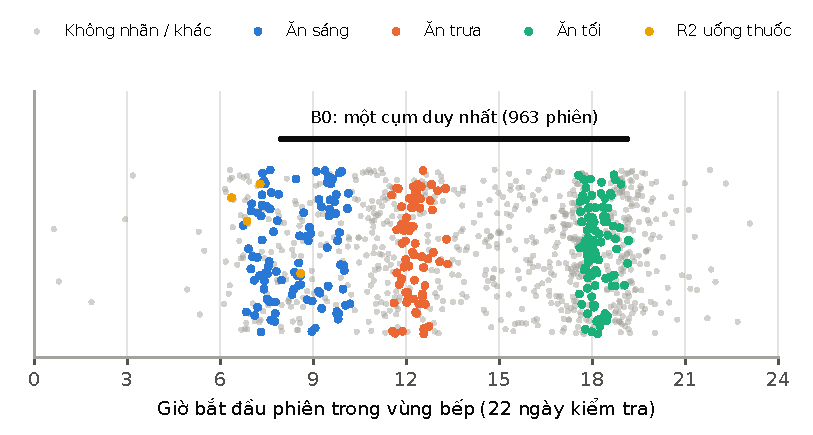
\includegraphics[width=\textwidth]{b0_kitchen_sessions}
\caption{Phiên trong vùng bếp của Cairo theo giờ bắt đầu (22 ngày kiểm tra), tô màu theo nhãn thật.
Phương pháp thực tập (B0) gộp toàn bộ thành một cụm duy nhất.}
\label{fig:b0}
\end{figure}

Ba bữa ăn tách bạch rõ ràng theo giờ, nhưng giữa chúng có rất nhiều phiên ngắn không nhãn --- hai người
đi lại xen kẽ khiến phiên bị cắt vụn (trung vị chỉ khoảng 2 phút). Các phiên này nối các bữa ăn lại với
nhau, và DBSCAN của phương pháp thực tập ``chuỗi hóa'' toàn bộ thành \textbf{một cụm 963 phiên trải từ
khoảng 8 giờ đến 19 giờ}. Thói quen uống thuốc của R2 --- chỉ vài phiên ngắn lẫn trong bữa sáng --- hoàn
toàn không thể tách ra. Đây không phải do thiếu nhãn mà là giới hạn của cách biểu diễn ``vùng × giờ''
khi trong nhà có hai người.

\section{RQ1 -- Nhận dạng (người, hoạt động)}
\label{sec:exp-rq1}

\begin{table}[htbp]
\centering
\caption{RQ1 -- F1 nhận dạng (người, hoạt động) theo sự kiện trên tập kiểm tra}
\label{tab:rq1}
\small
\begin{tabular}{lrrrrrr}
\toprule
Nhà & B2 macro-F1 & M1 macro-F1 & M2 macro-F1 & B2 micro-F1 & M1 micro-F1 & M2 micro-F1 \\
\midrule
Cairo & 0{,}32 & 0{,}41 & 0{,}38 & 0{,}49 & 0{,}57 & 0{,}40 \\
Tulum1 & 0{,}34 & 0{,}44 & 0{,}44 & 0{,}45 & 0{,}54 & 0{,}52 \\
Tulum2 & 0{,}40 & 0{,}48 & 0{,}46 & 0{,}49 & 0{,}57 & 0{,}55 \\
Milan & 0{,}35 & 0{,}49 & 0{,}47 & 0{,}59 & 0{,}69 & 0{,}67 \\
Aruba & 0{,}27 & 0{,}48 & 0{,}46 & 0{,}63 & 0{,}76 & 0{,}76 \\
\bottomrule
\end{tabular}
\end{table}


\begin{figure}[htbp]
\centering
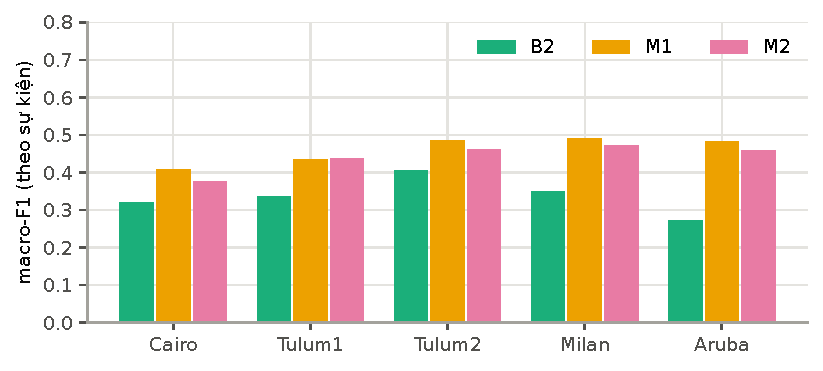
\includegraphics[width=0.85\textwidth]{rq1_macro_f1}
\caption{RQ1 -- macro-F1 theo sự kiện trên tập kiểm tra.}
\label{fig:rq1}
\end{figure}

Bảng~\ref{tab:rq1} và Hình~\ref{fig:rq1} cho thấy \textbf{hai mô hình học (M1, M2) vượt baseline tra
bảng B2 ở mọi nhà}, với chênh lệch macro-F1 từ 0,06 (Cairo, Tulum2) đến 0,21 (Aruba). M1 (Random
Forest) cao hơn M2 (Bi-GRU) ở bốn trên năm nhà; chỉ ở Tulum1 M2 nhỉnh hơn không đáng kể (0,438 so với
0,435). Mô hình chuỗi phức tạp hơn không mang lại lợi thế trên dữ liệu này --- phù hợp với việc Bi-GRU có
dấu hiệu học quá khớp ngay từ epoch thứ hai (Phụ lục~\ref{app:gru}).

Giá trị tuyệt đối (macro-F1 khoảng 0,38--0,49) thấp hơn nhiều so với các con số 80--90\% thường được báo
cáo trong tài liệu, kể cả trong~\cite{chen2021thesis}. Có ba lý do: (i) khóa luận \emph{chia theo thời
gian}, không xáo trộn; (ii) mỗi sự kiện được đánh giá với đầy đủ các hoạt động, kể cả các sự kiện không
thuộc hoạt động nào (chiếm phần lớn thời gian ở Cairo); (iii) Cairo, Tulum là nhà hai người với hoạt
động gắn người.

\begin{table}[htbp]
\centering
\caption{RQ1 -- F1 theo từng hoạt động trên Cairo}
\label{tab:rq1-cairo}
\small
\begin{tabular}{lrrr}
\toprule
Hoạt động & B2 & M1 & M2 \\
\midrule
Bed\_to\_Toilet & 0{,}30 & 0{,}16 & 0{,}22 \\
Breakfast & 0{,}42 & 0{,}51 & 0{,}57 \\
Dinner & 0{,}69 & 0{,}77 & 0{,}68 \\
Leave\_Home & 0{,}00 & 0{,}10 & 0{,}01 \\
Lunch & 0{,}55 & 0{,}65 & 0{,}60 \\
Night\_Wandering & 0{,}51 & 0{,}40 & 0{,}49 \\
R1\_Sleep & 0{,}05 & 0{,}35 & 0{,}30 \\
R1\_Wake & 0{,}35 & 0{,}56 & 0{,}46 \\
R1\_Work & 0{,}03 & 0{,}18 & 0{,}12 \\
R2\_Sleep & 0{,}49 & 0{,}41 & 0{,}42 \\
R2\_Take\_Medicine & 0{,}00 & 0{,}11 & 0{,}03 \\
R2\_Wake & 0{,}43 & 0{,}68 & 0{,}61 \\
\bottomrule
\end{tabular}
\end{table}


Bảng~\ref{tab:rq1-cairo} chi tiết theo hoạt động trên Cairo. Các bữa ăn và thức dậy đạt F1 0,5--0,8.
\textbf{Uống thuốc của R2 chỉ đạt 0,11} với M1: đây là hoạt động rất ngắn (trung vị 1,2 phút), diễn ra
ở đúng cảm biến bếp và cùng khung giờ với bữa sáng. ``Rời nhà'' (\texttt{Leave\_Home}) gần như không
nhận ra được vì hầu như không có sự kiện chuyển động nào trong lúc vắng nhà.

\section{RQ2 -- Thói quen của từng người}
\label{sec:exp-rq2}

\begin{table}[htbp]
\centering
\caption{RQ2 -- F1 thói quen theo nhà và phương pháp}
\label{tab:rq2-f1}
\small
\begin{tabular}{lrrrrrr}
\toprule
Phương pháp & Cairo & Tulum1 & Tulum2 & Milan & Aruba & Trung bình \\
\midrule
B0 & 0{,}24 & 0{,}22 & 0{,}33 & 0{,}38 & 0{,}29 & 0{,}29 \\
B1 & 0{,}12 & 0{,}22 & 0{,}18 & 0{,}38 & 0{,}27 & 0{,}23 \\
B2+H & 0{,}43 & 0{,}59 & 0{,}54 & 0{,}40 & 0{,}63 & 0{,}52 \\
M1+H & 0{,}62 & 0{,}71 & 0{,}50 & 0{,}54 & 0{,}59 & 0{,}59 \\
M2+H & 0{,}37 & 0{,}75 & 0{,}51 & 0{,}55 & 0{,}50 & 0{,}54 \\
Oracle+H & 1{,}00 & 1{,}00 & 1{,}00 & 1{,}00 & 1{,}00 & 1{,}00 \\
\bottomrule
\end{tabular}
\end{table}


\begin{figure}[htbp]
\centering
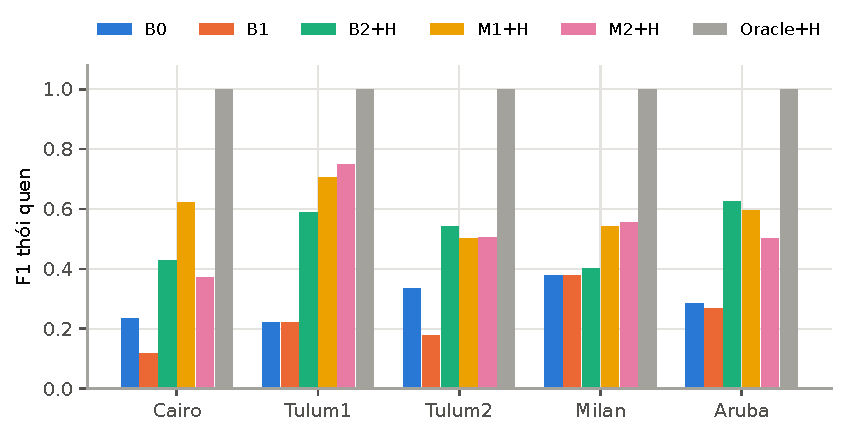
\includegraphics[width=\textwidth]{rq2_habit_f1}
\caption{RQ2 -- F1 của thói quen tìm được so với thói quen đáp án.}
\label{fig:rq2}
\end{figure}

Bảng~\ref{tab:rq2-f1} và Hình~\ref{fig:rq2} là kết quả trung tâm của khóa luận.

\textbf{(1) Học (người, hoạt động) rồi áp định nghĩa thói quen tốt hơn hẳn phương pháp theo vùng.} Trên
cả ba nhà hai người, M1+H đạt F1 thói quen 0,50--0,71 (M2+H: 0,37--0,75), trong khi B0 chỉ đạt
0,22--0,33. Khác biệt
nằm chủ yếu ở \emph{recall}: B0 tìm được rất ít thói quen có nghĩa (recall 0,17--0,22) vì các thói quen
bị gộp như mục~\ref{sec:exp-b0}.

\textbf{(2) Thói quen từng người ở Cairo.} Bảng~\ref{tab:rq2-cairo} và Hình~\ref{fig:timeline} chi tiết
Cairo. \textbf{M1+H tìm được đủ 6/6 thói quen gắn người}, trong đó có ``R2 uống thuốc 06:57'' (đáp án
07:08, ngày thường) --- đúng ví dụ mở đầu khóa luận. B0 chỉ tìm được 2/6, với khung giờ rộng hàng chục
giờ.

\begin{table}[htbp]
\centering
\caption{RQ2 -- So khớp thói quen với đáp án trên Cairo}
\label{tab:rq2-cairo}
\small
\begin{tabular}{lrrrrcc}
\toprule
Phương pháp & P & R & F1 & Lệch giờ (phút) & Khớp/đáp án & Từng người \\
\midrule
B0 & 0{,}25 & 0{,}22 & 0{,}24 & 32{,}03 & 2/9 & 2/6 \\
B1 & 0{,}13 & 0{,}11 & 0{,}12 & 31{,}49 & 1/9 & 0/6 \\
B2+H & 0{,}32 & 0{,}67 & 0{,}43 & 29{,}97 & 6/9 & 3/6 \\
M1+H & 0{,}45 & 1{,}00 & 0{,}62 & 13{,}19 & 9/9 & 6/6 \\
M2+H & 0{,}24 & 0{,}89 & 0{,}37 & 22{,}17 & 8/9 & 5/6 \\
Oracle+H & 1{,}00 & 1{,}00 & 1{,}00 & 0{,}00 & 9/9 & 6/6 \\
\bottomrule
\end{tabular}
\end{table}


\begin{figure}[htbp]
\centering
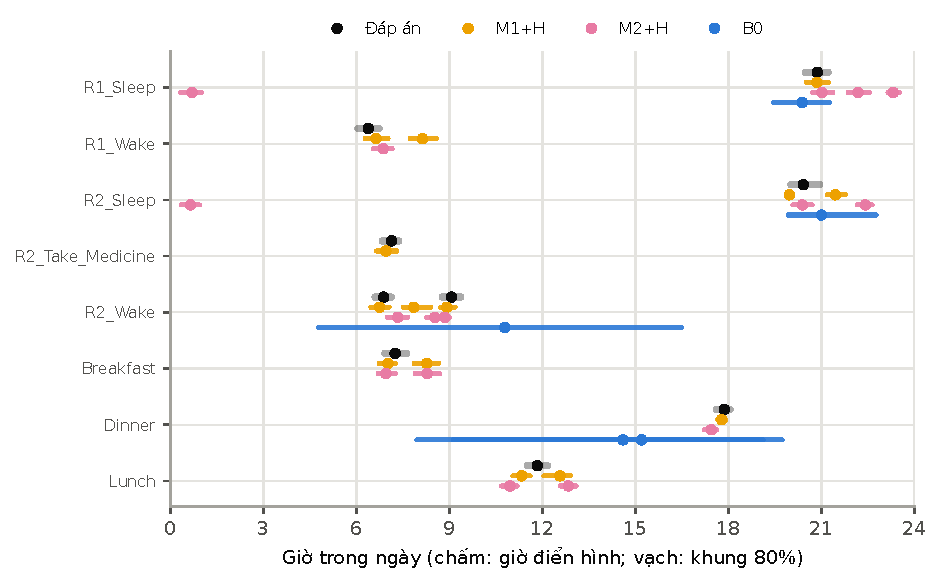
\includegraphics[width=\textwidth]{habits_timeline_cairo}
\caption{Thói quen trên Cairo: đáp án (đen), M1+H, M2+H và B0. Chấm là giờ điển hình, vạch là khung 80\%.}
\label{fig:timeline}
\end{figure}

\textbf{(3) Tách vệt theo vị trí (B1) không giúp, thậm chí làm tệ hơn.} Ở Cairo, B1 đạt 0,12 so với 0,24
của B0; ở Tulum2 là 0,18 so với 0,33. Heuristic ``sự kiện xa nhau thuộc hai người'' cắt vụn thêm các
phiên (số phiên tăng từ 2.748 lên 4.219 ở Cairo) mà không gắn được phiên với \emph{người cụ thể}: hai vệt
là vô danh và có thể đổi vai cho nhau theo thời gian. Kết quả này cho thấy, ít nhất với cảm biến chuyển
động thưa, \emph{tách người không cần nhãn} chưa đủ để học thói quen từng người; cần một tín hiệu học có
giám sát như ở M1, M2.

\textbf{(4) Khi thói quen chủ yếu gắn với ``vùng + giờ'', tra bảng đã khá tốt.} Ở Tulum2, B2+H (0,54)
ngang M1+H (0,50) và M2+H (0,51); ở Aruba (nhà một người), B2+H còn cao nhất (0,63 so với 0,59 của
M1+H). Phần lớn thói quen của Tulum2 là hoạt động chung lặp lại nhiều lần trong ngày (vệ sinh, xem
TV, làm việc), gắn chặt với ``vùng nào, khung giờ nào''. Ưu thế của mô hình học thể hiện rõ nhất ở các
hoạt động gắn người và hoạt động ngắn, như ở Cairo.

\textbf{(5) Lỗi chính của mô hình học là thói quen giả, không phải bỏ sót.} Ở mọi nhà, recall của M1+H và
M2+H cao (0,68--1,00) nhưng precision chỉ khoảng 0,24--0,60. Bảng~\ref{tab:false-cairo} truy ngược 11 thói
quen giả của M1+H trên Cairo: với mỗi thói quen giả, các lần thực hiện tạo nên nó được đối chiếu với nhãn
thật trùng thời gian. Hai nguồn lỗi hiện ra rõ:
\begin{itemize}
  \item \emph{Thói quen ``lệch bóng''} nằm ngay cạnh một thói quen thật của cùng hoạt động (ăn sáng 08:16
  cạnh 07:15; ăn trưa 12:34 cạnh 11:50; R2 thức dậy 07:51 cạnh 06:53; R2 ngủ 21:27 cạnh 20:25): bộ nhận dạng
  tiếp tục báo hoạt động sau khi nó đã kết thúc, đều đặn mỗi ngày, nên phần ``đuôi'' này tự thành một thói
  quen thứ hai.
  \item \emph{Khoảng không có nhãn}: ở 8/11 thói quen giả (kể cả phần lớn các thói quen lệch bóng ở trên),
  đa số các lần thực hiện rơi vào khoảng thời gian không có nhãn nào. Cairo chỉ được gán nhãn khoảng 2,5 giờ mỗi ngày, nên một phần các thói quen này có thể
  là hoạt động thật mà người chú thích không ghi (ví dụ các lần ``rời nhà'' 09:41, 13:01, 15:15).
\end{itemize}
Chỉ một trường hợp là nhầm hoạt động rõ ràng (``R1 làm việc 21:26'' trùng giờ R1 đi ngủ). Cả hai nguồn lỗi
chính đều là lỗi \emph{có hệ thống} --- lặp lại cùng một kiểu, cùng một giờ, ngày nào cũng như ngày nào ---
nên đủ nhiều để vượt ngưỡng 50\% số ngày. Mục~\ref{sec:exp-prop} sẽ cho thấy lỗi \emph{ngẫu nhiên} thì gần
như vô hại.

\begin{table}[htbp]
\centering
\caption{Thói quen giả của M1+H trên Cairo: mỗi dòng truy các lần thực hiện tạo nên thói quen về nhãn thật trùng thời gian}
\label{tab:false-cairo}
\small
\begin{tabular}{lccl}
\toprule
Thói quen giả & Số ngày & Thói quen thật gần nhất & Nhãn thật trùng nhiều nhất \\
\midrule
Ăn sáng 08:16 & 15 & 07:15 (lệch 61 phút) & (không nhãn) (11/18) \\
Rời nhà 09:41 & 4 & không có & (không nhãn) (6/9) \\
Rời nhà 13:01 & 4 & không có & (không nhãn) (7/8) \\
Rời nhà 15:15 & 4 & không có & (không nhãn) (5/5) \\
Ăn trưa 12:34 & 13 & 11:50 (lệch 44 phút) & (không nhãn) (10/14) \\
Đi lại ban đêm 00:56 & 14 & không có & (không nhãn) (7/16) \\
Đi lại ban đêm 03:50 & 16 & không có & Đi lại ban đêm (7/17) \\
R1 thức dậy 08:08 & 11 & 06:23 (lệch 105 phút) & R1 thức dậy (5/12) \\
R1 làm việc 21:26 & 4 & không có & R1 ngủ (4/11) \\
R2 ngủ 21:27 & 16 & 20:25 (lệch 61 phút) & (không nhãn) (13/21) \\
R2 thức dậy 07:51 & 12 & 06:53 (lệch 59 phút) & (không nhãn) (7/13) \\
\bottomrule
\end{tabular}
\end{table}


\textbf{(6) B0 bảo thủ: ít sai nhưng bỏ sót nhiều.} Ở Milan, Aruba và Tulum2, những thói quen B0 tìm ra
phần lớn là đúng (precision 0,64--0,75), nhưng nó chỉ tìm được 18--27\% số thói quen đáp án. Ở Cairo và
Tulum1 --- hai nhà mà hoạt động của hai người chồng lấn mạnh trong cùng vùng bếp --- precision của B0 cũng
giảm còn 0,25--0,33. Ngay ở nhà một người, M1+H và M2+H vẫn vượt B0 (0,50--0,59 so với 0,29--0,38): đơn
vị ``phiên trong vùng'' quá thô cho thói quen gắn với \emph{hoạt động}.

\section{Phân tích lỗi lan truyền}
\label{sec:exp-prop}

\begin{figure}[htbp]
\centering
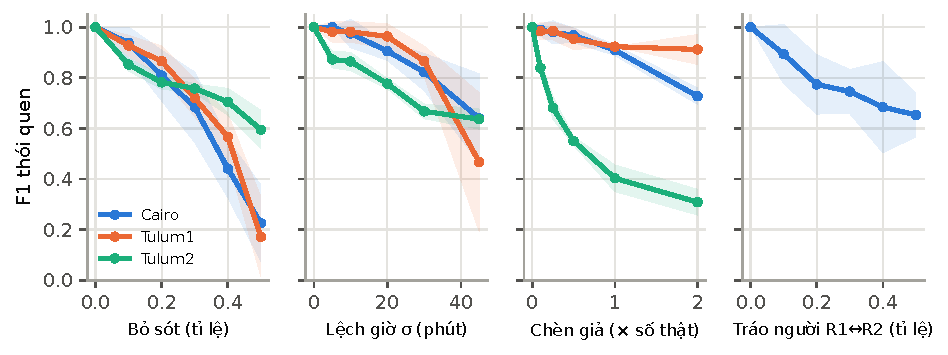
\includegraphics[width=\textwidth]{propagation}
\caption{F1 thói quen khi làm nhiễu nhãn thật có kiểm soát (trung bình $\pm$ độ lệch chuẩn qua 5 hạt
giống). Đường ``tráo người'' chỉ vẽ cho nhà có ít nhất 3 thói quen gắn người (Cairo).}
\label{fig:prop}
\end{figure}

Hình~\ref{fig:prop} trả lời phần thứ hai của RQ2: \emph{nhận dạng sai bao nhiêu thì thói quen sai bấy
nhiêu?}

\begin{itemize}
  \item \textbf{Bỏ sót là nguy hiểm nhất.} Vì thói quen cần xuất hiện ở ít nhất 50\% số ngày, bỏ sót đẩy
  tần suất xuống dưới ngưỡng. Ở Cairo, bỏ sót 20\% số lần thực hiện làm F1 còn 0,81; bỏ sót 40\% còn 0,44.
  \item \textbf{Lệch giờ gần như vô hại khi nhỏ.} Lệch chuẩn 10 phút giữ F1 ở 0,98 (Cairo); chỉ khi lệch
  từ 30 phút trở lên --- bằng nửa bề rộng cửa sổ --- F1 mới giảm rõ.
  \item \textbf{Chèn giả ngẫu nhiên ít ảnh hưởng}, đến khi số lần giả bằng số lần thật (Cairo: 0,91). Lỗi
  ngẫu nhiên rải đều trong ngày nên không tạo được đỉnh đạt 50\% số ngày. Đối chiếu với kết quả (5) ở
  mục~\ref{sec:exp-rq2}: \emph{lỗi có hệ thống} của bộ nhận dạng mới sinh thói quen giả.
  \item \textbf{Tráo người} R1$\leftrightarrow$R2 với xác suất 20\% làm F1 thói quen gắn người của Cairo
  còn 0,77. Một thói quen gắn người chịu được mức nhầm người vừa phải vì lần thực hiện đúng người vẫn
  chiếm đa số, nhưng thói quen sát ngưỡng bị mất trước.
  \item \textbf{Độ bền phụ thuộc khoảng cách tới ngưỡng.} Tulum2 nhạy hơn hẳn Cairo với mọi loại lỗi
  (chèn giả 10\% đã còn 0,84): thói quen của Tulum2 là các hoạt động lặp nhiều lần với tần suất chỉ vừa
  qua 50\%, nên một chút nhiễu đủ đẩy chúng qua lại ngưỡng.
\end{itemize}

\textbf{Hàm ý thực tế.} Để học thói quen, một bộ nhận dạng cần ưu tiên \emph{không bỏ sót} và \emph{không
nhầm có hệ thống}; sai lệch giờ nhỏ và nhận thừa rải rác là chấp nhận được. Điều này khác với tiêu chí
accuracy/F1 theo sự kiện thường dùng để tối ưu mô hình nhận dạng.

\section{Ablation và độ nhạy}
\label{sec:exp-ablation}

\begin{table}[htbp]
\centering
\caption{Ablation -- F1 thói quen khi thay một thành phần (dòng ``Nhãn thật'': khai phá trên nhãn thật của ngày kiểm tra)}
\label{tab:ablation}
\small
\begin{tabular}{llrrrrr}
\toprule
Đầu vào & Biến thể & Cairo & Tulum1 & Tulum2 & Milan & Aruba \\
\midrule
Nhãn thật & Quét cửa sổ (mặc định) & 1{,}00 & 1{,}00 & 1{,}00 & 1{,}00 & 1{,}00 \\
Nhãn thật & DBSCAN & 0{,}90 & 0{,}92 & 0{,}63 & 0{,}77 & 0{,}38 \\
Nhãn thật & HDBSCAN & 0{,}61 & 0{,}22 & 0{,}50 & 0{,}75 & 0{,}52 \\
Nhãn thật & Không tách loại ngày & 0{,}71 & 1{,}00 & 0{,}56 & 0{,}79 & 0{,}71 \\
\midrule
M1 & Mặc định (quét cửa sổ, nối 10 phút) & 0{,}62 & 0{,}71 & 0{,}50 & 0{,}54 & 0{,}59 \\
M1 & DBSCAN & 0{,}64 & 0{,}53 & 0{,}51 & 0{,}52 & 0{,}08 \\
M1 & HDBSCAN & 0{,}41 & 0{,}53 & 0{,}37 & 0{,}60 & 0{,}53 \\
M1 & Không tách loại ngày & 0{,}67 & 0{,}71 & 0{,}49 & 0{,}54 & 0{,}50 \\
\midrule
M1 & Khoảng nối 2 phút & 0{,}69 & 0{,}71 & 0{,}61 & 0{,}56 & 0{,}38 \\
M1 & Khoảng nối 5 phút & 0{,}64 & 0{,}75 & 0{,}60 & 0{,}53 & 0{,}45 \\
M1 & Khoảng nối 20 phút & 0{,}67 & 0{,}71 & 0{,}47 & 0{,}61 & 0{,}32 \\
M1 & Khoảng nối 30 phút & 0{,}62 & 0{,}75 & 0{,}43 & 0{,}68 & 0{,}33 \\
\bottomrule
\end{tabular}
\end{table}


\textbf{Thuật toán khai phá.} Trên nhãn thật (dòng ``Oracle''), DBSCAN chỉ khớp định nghĩa ở mức F1
0,38--0,92 và HDBSCAN ở mức 0,22--0,75 tùy nhà: DBSCAN chuỗi hóa các hoạt động lặp nhiều lần (chỉ còn 0,38
ở Aruba), HDBSCAN không có khái niệm ``lệch không quá 30 phút''. Đây là căn cứ để khóa luận hiện thực định
nghĩa bằng thuật toán quét cửa sổ thay vì HDBSCAN như dự kiến ban đầu. Trên đầu ra của M1, quét cửa sổ tốt
nhất ở Tulum1 và Aruba (DBSCAN chỉ còn 0,08 ở Aruba), chênh không quá 0,02 so với DBSCAN ở Cairo, Milan và
Tulum2; HDBSCAN cao hơn ở Milan (0,60 so với 0,54) nhưng thấp hơn rõ ở Cairo và Tulum2. Ưu điểm chính của
quét cửa sổ là \emph{đúng định nghĩa} và \emph{không sụp} ở bất kỳ nhà nào.

\textbf{Tách ngày thường -- cuối tuần.} Kết quả lẫn lộn: bỏ bước này làm F1 của M1 giảm ở Aruba (0,59
$\rightarrow$ 0,50), tăng ở Cairo (0,62 $\rightarrow$ 0,67) và gần như không đổi ở ba nhà còn lại. Với số
ngày kiểm tra ít (6--16 ngày cuối tuần ở các nhà nhỏ), thói quen riêng cuối tuần dễ là thói quen giả; với
nhà có nhiều ngày như Aruba (88 ngày kiểm tra), bước này giúp ích. Bước này hữu ích khi đáp án có thói quen riêng cuối tuần rõ ràng (``R2 dậy
muộn 9:04 cuối tuần'' ở Cairo) nhưng cần nhiều ngày hơn để ổn định.

\textbf{Khoảng nối khi giải mã.} Khoảng nối là tham số nhạy: ở Aruba, F1 của M1 dao động 0,32--0,59 (tốt nhất
ở 10 phút); ở các nhà khác dao động đến 0,2 và không có giá trị tốt nhất chung (Tulum2 thích khoảng ngắn,
Milan thích khoảng dài). Đây là điểm cần cải tiến: bước giải mã nên xét thời lượng điển hình của từng hoạt
động thay vì một khoảng nối chung.

\begin{table}[htbp]
\centering
\caption{Độ nhạy -- F1 thói quen trung bình năm nhà khi đổi tham số định nghĩa}
\label{tab:sensitivity}
\small
\begin{tabular}{rrrrrrr}
\toprule
Cửa sổ $\pm$(phút) & Ngưỡng & B0 & B1 & B2+H & M1+H & M2+H \\
\midrule
15 & 0{,}40 & 0{,}26 & 0{,}20 & 0{,}43 & 0{,}50 & 0{,}46 \\
15 & 0{,}50 & 0{,}28 & 0{,}26 & 0{,}32 & 0{,}38 & 0{,}35 \\
15 & 0{,}60 & 0{,}19 & 0{,}19 & 0{,}35 & 0{,}33 & 0{,}35 \\
30 & 0{,}40 & 0{,}28 & 0{,}23 & 0{,}51 & 0{,}64 & 0{,}57 \\
30 & 0{,}50 & 0{,}29 & 0{,}23 & 0{,}52 & 0{,}59 & 0{,}54 \\
30 & 0{,}60 & 0{,}28 & 0{,}22 & 0{,}44 & 0{,}52 & 0{,}44 \\
45 & 0{,}40 & 0{,}31 & 0{,}26 & 0{,}50 & 0{,}61 & 0{,}55 \\
45 & 0{,}50 & 0{,}31 & 0{,}25 & 0{,}54 & 0{,}64 & 0{,}59 \\
45 & 0{,}60 & 0{,}30 & 0{,}22 & 0{,}53 & 0{,}58 & 0{,}52 \\
\bottomrule
\end{tabular}
\end{table}


\textbf{Độ nhạy theo định nghĩa.} Bảng~\ref{tab:sensitivity} thay đồng thời tham số của định nghĩa cho cả
đáp án và dự đoán. Với cửa sổ $\pm 30$ và $\pm 45$ phút, thứ tự trung bình các phương pháp ổn định: M1+H $>$ M2+H $\approx$
B2+H $>$ B0 $>$ B1. Với cửa sổ hẹp $\pm 15$ phút, mọi phương pháp giảm mạnh và khoảng cách giữa mô hình học
và tra bảng gần như biến mất ---
cửa sổ hẹp hơn sai số giờ bắt đầu của bộ nhận dạng. Định nghĩa $\pm 30$ phút là điểm cân bằng hợp lý giữa
``đủ chặt để có nghĩa'' và ``đủ rộng để học được''.

\section{RQ3 -- Phát hiện ngày bỏ thuốc}
\label{sec:exp-rq3}

\begin{table}[htbp]
\centering
\caption{RQ3 -- Phát hiện ngày bỏ thuốc \texttt{R2\_Take\_Medicine} trên Cairo (trung bình 5 lần cài; F1 ghi trung bình $\pm$ độ lệch chuẩn)}
\label{tab:rq3}
\small
\begin{tabular}{lrrcr}
\toprule
Bộ phát hiện & P & R & F1 & Báo nhầm/ngày \\
\midrule
B0-vùng & 0{,}00 & 0{,}00 & 0{,}00 $\pm$ 0{,}00 & 0{,}00 \\
B2 & 0{,}20 & 1{,}00 & 0{,}33 $\pm$ 0{,}00 & 0{,}80 \\
M1 & 0{,}00 & 0{,}00 & 0{,}00 $\pm$ 0{,}00 & 0{,}00 \\
M2 & 0{,}25 & 0{,}90 & 0{,}39 $\pm$ 0{,}10 & 0{,}54 \\
\bottomrule
\end{tabular}
\end{table}


\begin{figure}[htbp]
\centering
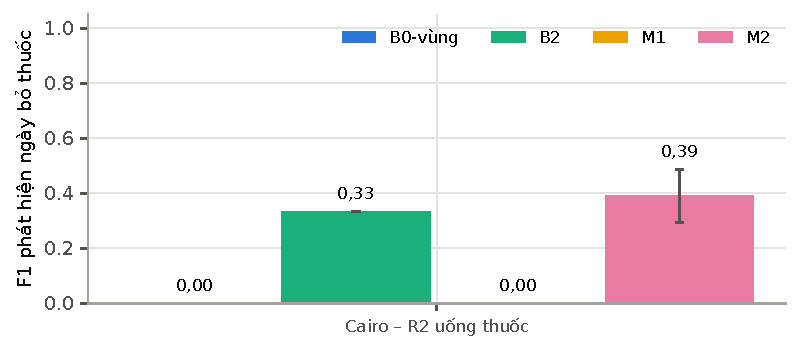
\includegraphics[width=0.75\textwidth]{rq3_detection}
\caption{RQ3 -- F1 phát hiện ngày bỏ thuốc trên Cairo (trung bình $\pm$ độ lệch chuẩn qua 5 lần cài).}
\label{fig:rq3}
\end{figure}

\textbf{Thiết lập thực tế.} Thói quen chuẩn ``R2 uống thuốc'' học từ ngày huấn luyện có cửa sổ phát hiện
06:19--07:58. Trong 22 ngày kiểm tra của Cairo, \textbf{12 ngày không có nhãn uống thuốc nào trong cửa
sổ} --- không thể biết R2 bỏ thuốc thật hay người chú thích không ghi. Những ngày này bị loại khỏi chấm
điểm, còn 10 ngày; mỗi lần cài chọn 2 ngày làm ngày bỏ thuốc. Ở Milan, giờ uống thuốc trong giai đoạn huấn
luyện dao động quá rộng (thuốc sáng khoảng 08:06--10:25; thuốc tối chỉ có nhãn 5/37 ngày) nên không tạo
được thói quen chuẩn theo định nghĩa; RQ3 vì vậy chỉ đánh giá được trên Cairo.

\textbf{Kết quả} (Bảng~\ref{tab:rq3}, Hình~\ref{fig:rq3}):
\begin{itemize}
  \item \textbf{B0-vùng và M1 không bao giờ báo động.} Khi xóa sự kiện uống thuốc, vùng bếp vẫn có người
  (bữa sáng), nên B0-vùng luôn thấy ``bình thường''. M1 cũng vẫn ``thấy'' uống thuốc: Random Forest học
  ngữ cảnh ``bếp, khoảng 7 giờ'' chứ không học dấu hiệu riêng của việc uống thuốc. Đây chính là lỗi có
  hệ thống đã nói ở mục~\ref{sec:exp-rq2}.
  \item \textbf{M2 phát hiện 9/10 ngày bỏ thuốc} (tổng qua 5 lần cài; recall 0,90) nhưng báo động nhầm
  0,54 lần mỗi ngày.
  Mô hình chuỗi nhạy hơn với việc thiếu một đoạn sự kiện ngắn, đổi lại kém ổn định.
  \item B2 báo động gần như mọi ngày (recall 1,0, precision 0,2) nên không có giá trị sử dụng.
\end{itemize}
Vì bộ phát hiện chờ hết cửa sổ (07:58) mới kết luận, báo động đến khoảng 47 phút sau giờ uống thuốc điển
hình --- đủ sớm để nhắc trong cùng buổi sáng.

\textbf{Nhận định.} RQ3 cho câu trả lời \emph{một phần}: thói quen học được \emph{có} chứa thông tin để
phát hiện bỏ thuốc (M2), và tốt hơn hẳn cách theo vùng (vốn không thể phát hiện), nhưng chưa đủ tin cậy
để dùng thực tế: số báo động nhầm còn cao và mẫu đánh giá nhỏ (10 ngày dương tính qua 5 lần cài). Kết
quả này cũng cho thấy một điểm đáng chú ý: \emph{mô hình tốt hơn ở RQ2 (M1) lại kém hơn ở RQ3}, vì phát
hiện ``vắng mặt'' đòi hỏi mô hình dựa vào dấu hiệu riêng của hoạt động chứ không dựa vào ngữ cảnh.

\section{Thảo luận}
\label{sec:exp-discussion}

\textbf{Trả lời ba câu hỏi nghiên cứu.}
\begin{description}[leftmargin=1.2cm,style=sameline]
  \item[RQ1] Gán (người, hoạt động) theo sự kiện đạt macro-F1 khoảng 0,38--0,49 với mô hình học khi đánh
  giá theo thời gian; mô hình học vượt tra bảng ở mọi nhà. Hoạt động ngắn, trùng chỗ (uống thuốc) và hoạt
  động ít sự kiện (rời nhà) là khó nhất.
  \item[RQ2] Dù nhận dạng theo sự kiện còn thấp, thói quen tìm được vẫn tốt hơn hẳn phương pháp theo vùng:
  F1 0,50--0,71 (M1+H) so với 0,22--0,33 ở nhà hai người, và đủ 6/6 thói quen gắn người ở Cairo. Thói quen
  \emph{chịu được} lệch giờ nhỏ và nhận thừa ngẫu nhiên, nhưng \emph{nhạy} với bỏ sót, nhầm người và lỗi
  có hệ thống.
  \item[RQ3] Có thể phát hiện ngày bỏ thuốc ở mức nhất định (M2: recall 0,9), nhưng báo động nhầm còn cao;
  cách theo vùng hoàn toàn không phát hiện được.
\end{description}

\textbf{Mối đe dọa tính hợp lệ.}
\begin{itemize}
  \item \emph{Số thói quen gắn người nhỏ} (6 ở Cairo, 1 ở mỗi nhà Tulum): kết luận về ``từng người'' chủ
  yếu dựa trên Cairo.
  \item \emph{Nhãn thưa}: Cairo chỉ gán nhãn khoảng 2,5 giờ mỗi ngày; một thói quen ``giả'' có thể là thói
  quen thật mà người chú thích không ghi.
  \item \emph{Một lần chia dữ liệu}: kết quả dựa trên một lần chia 60/40 theo thời gian; chưa có khoảng tin
  cậy theo nhiều lần chia (dự kiến bổ sung ở bản v2).
  \item \emph{Gán nhãn cho cụm B0, B1 dùng nhãn tập kiểm tra}: có lợi cho baseline; so sánh vì thế thận trọng.
  \item \emph{Bất thường được cài}: ngày bỏ thuốc thật có thể để lại dấu vết khác (ví dụ không mở tủ thuốc
  nhưng vẫn vào bếp lâu hơn).
\end{itemize}

\chapter{Kết luận và hướng phát triển}
\label{chap:conclusion}

\section{Kết luận}

Khóa luận nghiên cứu bài toán học thói quen sinh hoạt của \emph{từng người} trong nhà thông minh có
nhiều người, chỉ từ cảm biến môi trường --- nơi các sự kiện của hai người trộn vào một luồng vô danh.
Xuất phát từ đề tài thực tập (tìm thói quen cho nhà một người) và định hướng từ luận án của
Chen~\cite{chen2021thesis} (nhận dạng hoạt động trong nhà nhiều người), khóa luận đi tiếp theo hướng
luận án còn bỏ ngỏ: từ nhận dạng hoạt động hiện tại sang hành vi dài hạn.

Các kết quả chính:

\begin{enumerate}
  \item \textbf{Phương pháp theo vùng của đề tài thực tập không dùng được cho nhà hai người.} Trên Cairo,
  hai người đi lại xen kẽ làm phiên bị cắt vụn, và DBSCAN gộp toàn bộ các bữa ăn cùng việc uống thuốc
  trong vùng bếp thành một cụm duy nhất. Tách luồng theo vị trí (B1) không khắc phục được, thậm chí còn
  làm kết quả tệ hơn.
  \item \textbf{Học (người, hoạt động) rồi áp định nghĩa thói quen cho kết quả tốt hơn hẳn.} Ở ba nhà hai
  người, F1 thói quen của Random Forest đạt 0,50--0,71 so với 0,22--0,33 của phương pháp thực tập; ở Cairo, Random Forest
  tìm đủ 6/6 thói quen gắn người, trong đó có thói quen uống thuốc của R2 --- đúng trường hợp mà cách
  tiếp cận theo vùng không thể tách được.
  \item \textbf{Định nghĩa thói quen được hiện thực đúng nguyên văn} bằng thuật toán quét cửa sổ đếm theo
  ngày. Ablation cho thấy DBSCAN và HDBSCAN lệch khỏi định nghĩa đáng kể ngay cả trên nhãn thật.
  \item \textbf{Thói quen chịu được lệch giờ nhỏ và nhận thừa ngẫu nhiên, nhưng nhạy với bỏ sót, nhầm
  người và lỗi có hệ thống.} Lỗi chính của các mô hình hiện tại là thói quen giả sinh từ lỗi nhận dạng lặp
  lại đều đặn, không phải bỏ sót.
  \item \textbf{Phát hiện ngày bỏ thuốc khả thi một phần}: Bi-GRU phát hiện 9/10 ngày bỏ thuốc được cài
  nhưng còn nhiều báo động nhầm; cách tiếp cận theo vùng không phát hiện được ngày nào. Mô hình tốt nhất cho
  thói quen (Random Forest) lại không phát hiện được sự vắng mặt --- một bài học về sự khác nhau giữa
  ``nhận ra điều đang có'' và ``nhận ra điều đã không xảy ra''.
\end{enumerate}

\section{Hạn chế}

\begin{itemize}
  \item \textbf{Dữ liệu}: chỉ có ba nhà hai người, nhãn gắn người ít (đánh giá ``từng người'' chủ yếu dựa
  trên Cairo), nhãn thưa và dữ liệu thu từ 2009--2011 ở Mỹ.
  \item \textbf{Đánh giá}: số ngày kiểm tra mỗi lần chia ít nên kết quả dao động lớn; đánh giá qua nhiều lần
  chia mới làm cho ba nhà hai người; mẫu của RQ3 nhỏ và bất thường là bất thường được cài.
  \item \textbf{Phương pháp}: bộ nhận dạng chưa được tối ưu cho mục tiêu thói quen (ít bỏ sót, ít lỗi có hệ
  thống); bước giải mã còn đơn giản.
\end{itemize}

\section{Hướng phát triển}

\textbf{Hướng phát triển trực tiếp của khóa luận:}
\begin{enumerate}
  \item Mở rộng đánh giá qua nhiều lần chia cho cả năm nhà và với dữ liệu dài hơn, để thu hẹp độ dao động.
  \item Giảm thói quen giả: giải mã có xét thời lượng hoạt động, ràng buộc ``mỗi người mỗi ngày tối đa một
  lần thức dậy'', hoặc hiệu chỉnh ngưỡng theo mục tiêu thói quen thay vì F1 theo sự kiện.
  \item Giảm phụ thuộc vào giờ trong ngày của bộ nhận dạng (Hình~\ref{fig:rf-imp}), ví dụ bằng đặc trưng
  mô tả chuỗi chuyển động thay cho giờ, để mô hình nhận ra cả sự \emph{vắng mặt} của một hoạt động.
  \item Mở rộng dữ liệu nếu xin được: ARAS~\cite{alemdar2013aras}, CASAS Kyoto/twor.
\end{enumerate}

\textbf{Ngoài phạm vi khóa luận} (các ứng dụng xây trên nền thói quen):
\begin{itemize}
  \item Hệ thống nhắc uống thuốc thật, có giao diện cho người chăm sóc.
  \item Dự đoán hoạt động tiếp theo dựa trên thói quen~\cite{doctorarastoo2026prediction}.
  \item Dùng mô hình ngôn ngữ để giải thích thói quen và thay đổi hành vi cho gia đình hoặc bác
  sĩ~\cite{civitarese2026xbcd}, hoặc mô tả cảm biến bằng văn bản để chuyển sang nhà
  mới~\cite{thukral2024tdost,fiori2026domusfm}.
  \item Nhà từ ba người trở lên với dữ liệu như MuRAL~\cite{chen2025mural}.
\end{itemize}


% ---------------- Tài liệu tham khảo ----------------
\clearpage
\phantomsection
\addcontentsline{toc}{chapter}{Tài liệu tham khảo}
\renewcommand{\bibname}{Tài liệu tham khảo}
\bibliographystyle{ieeetr}
\bibliography{references}

% ---------------- Phụ lục ----------------
\appendix
\addtocontents{toc}{\protect\renewcommand{\protect\cftchappresnum}{Phụ lục\ }}
\addtocontents{toc}{\protect\setlength{\protect\cftchapnumwidth}{6.5em}}

\chapter{Chọn cấu hình Bi-GRU}
\label{app:gru}

Mô hình M2 có dấu hiệu học quá khớp ngay từ epoch thứ hai (mất mát huấn luyện giảm, mất mát kiểm định
tăng). Ba cấu hình được thử trên tập kiểm định của Cairo (25\% số ngày cuối của tập huấn luyện); cấu hình
có mất mát kiểm định nhỏ nhất được dùng cho mọi nhà. Tập kiểm tra không được dùng ở bước này.

\begin{table}[htbp]
\centering
\caption{Ba cấu hình Bi-GRU thử trên tập kiểm định Cairo}
\label{tab:gru-config}
\begin{tabular}{rrrrr}
\toprule
Số đơn vị ẩn & Dropout & Tốc độ học & Weight decay & Mất mát kiểm định \\
\midrule
\textbf{64} & \textbf{0,2} & $\mathbf{10^{-3}}$ & \textbf{0} & \textbf{0,3626} \\
32 & 0,3 & $5\cdot10^{-4}$ & $10^{-4}$ & 0,3645 \\
32 & 0,5 & $3\cdot10^{-4}$ & $10^{-3}$ & 0,3772 \\
\bottomrule
\end{tabular}
\end{table}

\chapter{Phân vùng thủ công của Cairo}
\label{app:cairo-zones}

Phân vùng dưới đây đọc từ sơ đồ mặt bằng chính thức~\cite{casas2025floorplans}, chỉ dùng để kiểm chứng
phân vùng tự động ở mục~\ref{sec:m-topo}; không được dùng trong bất kỳ phương pháp nào.

\begin{table}[htbp]
\centering
\caption{Bảy vùng của nhà Cairo theo sơ đồ mặt bằng}
\label{tab:cairo-manual}
\begin{tabular}{lll}
\toprule
Tầng & Vùng & Cảm biến \\
\midrule
Tầng chính & Bếp & M019, M020, M021, M022, M024 \\
           & Phòng khách -- ăn & M013, M016, M017, M018, M023 \\
           & Hành lang, cầu thang & M011, M012, M014, M015 \\
Tầng trên  & Phòng ngủ & M005, M006, M007, M008, M009 \\
           & Phòng trái & M001, M002, M003, M010 \\
           & Phòng phải & M004 \\
Tầng hầm   & Giặt là & M025, M026, M027 \\
\bottomrule
\end{tabular}
\end{table}

\chapter{Tái lập kết quả}
\label{app:repro}

Toàn bộ số liệu, bảng và hình trong khóa luận được sinh từ mã nguồn đi kèm. Sau khi cài đặt, các lệnh sau
lần lượt chạy thực nghiệm chính cho năm nhà, chạy đánh giá qua ba lần chia theo thời gian, sinh bảng và hình
cho khóa luận, và chạy bộ kiểm thử tự động:

\begin{center}
\begin{tabular}{@{}ll@{}}
\toprule
Lệnh & Tác dụng\\
\midrule
\verb|pip install -e ".[dev]"| & cài đặt gói mã nguồn và công cụ kiểm thử\\
\verb|python -m mrhabits.cli run| & thực nghiệm chính cho năm nhà\\
\verb|python -m mrhabits.cli rolling| & đánh giá qua ba lần chia theo thời gian\\
\verb|python -m mrhabits.cli figures| & sinh bảng và hình cho khóa luận\\
\verb|python -m pytest| & chạy bộ kiểm thử tự động\\
\bottomrule
\end{tabular}
\end{center}

Dữ liệu đặt tại \texttt{data/raw/casas/new\_labeled\_data.zip} (tải từ Zenodo, bản ghi 17180309). Các hạt
giống ngẫu nhiên được cố định (Random Forest: 0; Bi-GRU: 0; cài bất thường: 0--4; làm nhiễu nhãn: 1000--1004).
Cấu hình đầy đủ được ghi vào \texttt{results/config.json} mỗi lần chạy. Thực nghiệm chính mất khoảng một giờ
trên máy tính xách tay 12 luồng CPU, không dùng GPU.


\end{document}
